\documentclass[12pt,a4paper]{article}
\usepackage[margin=1in]{geometry}
\usepackage{graphicx}
\usepackage{amsmath}
\usepackage{booktabs}
\usepackage{fancyhdr}
\usepackage{setspace}
\usepackage{enumitem}
\usepackage{float}
\usepackage{xcolor}
\usepackage{amssymb}
\usepackage[colorlinks=true,linkcolor=blue,citecolor=blue,urlcolor=blue,bookmarks=true]{hyperref}

\hypersetup{
    pdftitle={Progress Report: EEG-Based Alzheimer's Disease Detection},
    pdfauthor={Arkidaroi Sama},
    pdfsubject={M.Tech Thesis Progress Report},
    pdfkeywords={EEG, Alzheimer's Disease, Welch PSD, CNN, OpenNeuro},
    bookmarksnumbered=true,
    bookmarksopen=true
}

\pagestyle{fancy}
\fancyhf{}
\fancyhead[L]{M.Tech Thesis Progress Report}
\fancyhead[R]{April 2026}
\fancyfoot[C]{\thepage}

\onehalfspacing

\begin{document}

% ==================== TITLE PAGE ====================
\begin{titlepage}
    \centering
    \vspace*{1cm}

    {\LARGE\bfseries M. TECH PROGRESS REPORT}\\[1cm]

    {\LARGE\bfseries ON}\\[1cm]

    {\huge\bfseries Comparative Evaluation of Convolutional Neural Networks for Alzheimer’s Disease Detection Using Welch-Based Frequency-Domain EEG Features}\\[2cm]

    {\large\textbf{Submitted by}}\\[0.3cm]
    {\Large Arkidaroi Sama}\\[0.2cm]
    {\large Roll Number: MTECHIT\_01}\\[2cm]

    {\large\textbf{Under the Supervision of}}\\[0.3cm]
    {\Large Mrs. Sangita Neog}\\

    \vfill

    {\large\textbf{Department of Information Technology}}\\
    {\large School of Technology}\\
    {\large North-Eastern Hill University}\\[1.5cm]

    {\large\textbf{April 01, 2026}}
\end{titlepage}

\tableofcontents
\newpage

% ==================== PROJECT OVERVIEW ====================
\section{Project Overview}

\subsection{Research Title}
Comparative Evaluation of Convolutional Neural Networks for Alzheimer’s Disease Detection Using Welch-Based Frequency-Domain EEG Features.

\subsection{Aim of the Project}
The aim of this project is to build an EEG-based pipeline for Alzheimer’s disease related analysis and to later compare multiple Convolutional Neural Network (CNN) architectures on frequency-domain EEG representations.

In the current phase of the work, the focus is on building a reliable and reproducible EEG preprocessing pipeline and extracting Welch Power Spectral Density (PSD) features from resting-state EEG recordings. These extracted features will serve as the input for CNN-based classification in the next phase of the thesis.

\subsection{Objectives}
\textbf{Phase 1 (Completed):}
\begin{itemize}[leftmargin=2em]
    \item Inspect the OpenNeuro \texttt{ds004504} dataset and identify valid EEG recordings.
    \item Create subject metadata using \texttt{participants.tsv}.
    \item Load and preprocess EEG signals using MNE.
    \item Segment the EEG into fixed-length epochs.
    \item Reject noisy or artifact-contaminated epochs using fixed rules.
    \item Extract frequency-domain features using Welch PSD.
    \item Save subject-wise PSD features and summary outputs for later use.
    \item Implement and compare non-overlapping (0\%) and 50\% overlapping epoch segmentation pipelines.
    \item Add a pilot single-CNN baseline workflow (EEGNet) for Phase 2 readiness.
\end{itemize}

\textbf{Phase 2 (Future Work):}
\begin{itemize}[leftmargin=2em]
    \item Create subject-wise train, validation, and test splits.
    \item Extend from the EEGNet pilot to full comparative modeling with ShallowConvNet, DeepConvNet, SCCNet, and FBCNet.
    \item Train and evaluate all selected models using a unified experimental setup.
    \item Compare model performance using standard evaluation metrics.
\end{itemize}

\subsection{Current Progress}
\begin{itemize}
    \item Current status: Phase 1 completed with overlap-comparison extension and EEGNet pilot implementation
    \item Completed scope: Dataset inspection, metadata creation, preprocessing, artifact rejection, epoch segmentation (0\% and 50\% overlap), Welch PSD extraction, output saving, progress visualization, and single-CNN baseline notebook integration
    \item Estimated progress: Approximately 55--60\%
\end{itemize}

\newpage

% ==================== LITERATURE REVIEW ====================
\section{Work Completed till Date}

\subsection{Literature Review}
A literature review was carried out to understand the present state of EEG-based Alzheimer’s disease detection and the role of deep learning in this area.

Resting-state EEG has been widely used in dementia research because it is non-invasive, relatively affordable, and sensitive to functional brain changes \cite{cassani2018,jeong2004,dauwels2010}. One of the most frequently reported EEG findings in Alzheimer’s disease is spectral slowing, where power tends to increase in lower-frequency bands and decrease in higher-frequency bands \cite{cassani2018,jeong2004,dauwels2010}. This makes frequency-domain analysis an important approach for disease-related EEG pattern analysis.

Many earlier studies used handcrafted EEG features together with classical machine learning methods such as Support Vector Machines and Random Forests \cite{cassani2018,tzimourta2019}. These studies achieved useful results, but their performance often depends heavily on feature engineering and dataset-specific choices.

More recent studies have explored deep learning, especially Convolutional Neural Networks, for EEG classification \cite{lawhern2018,schirrmeister2017,hsu2018,mane2021,roy2019,craik2019}. Architectures such as EEGNet, DeepConvNet, SCCNet, and FBCNet are attractive because they can learn structured patterns from EEG inputs \cite{lawhern2018,schirrmeister2017,hsu2018,mane2021}. However, many published works focus on one model at a time, or on raw EEG and time-domain representations, rather than performing a systematic comparison across multiple CNN models using a shared feature representation \cite{roy2019,craik2019}.

Based on this review, the present work is motivated by two points: first, Welch PSD provides an interpretable and widely accepted frequency-domain representation of EEG \cite{welch1967}; second, a comparative study of multiple CNN models using a common PSD-based input can provide a more structured evaluation framework for Alzheimer’s disease detection.

\subsection{Research Gap Identified}
The following research gaps motivated the current thesis:
\begin{itemize}
    \item many studies use EEG for dementia analysis, but do not evaluate multiple CNN architectures under a common experimental setup;
    \item frequency-domain EEG representations are important, but not always standardized across studies;
    \item subject-wise evaluation and leakage prevention are often not discussed clearly;
    \item publicly available datasets are available, but reproducible end-to-end pipelines are still needed before fair model comparison.
\end{itemize}

\subsection{Summary of Literature Position}
\begin{table}[H]
\centering
\scriptsize
\setlength{\tabcolsep}{2pt}
\renewcommand{\arraystretch}{1.2}
\begin{tabular}{|p{2.4cm}|p{1.9cm}|p{2.1cm}|p{2.1cm}|p{2.9cm}|}
\hline
\textbf{Author (Year)} & \textbf{Dataset Type} & \textbf{Method} & \textbf{Feature Style} & \textbf{Observation} \\
\hline
Lawhern et al. (2018) & EEG datasets & EEGNet & Compact learned filters & Strong baseline EEG CNN architecture \\
\hline
Schirrmeister et al. (2017) & EEG datasets & DeepConvNet / ShallowConvNet & Raw EEG / learned features & Effective deep CNNs for EEG decoding \\
\hline
Hsu et al. (2018) & EEG datasets & SCCNet & Spatial CNN features & Useful spatial modeling for EEG classification \\
\hline
Mane et al. (2021) & EEG datasets & FBCNet & Multi-view frequency features & Relevant for frequency-domain EEG learning \\
\hline
Welch (1967) & General signal processing & Welch PSD & Frequency-domain estimation & Standard method for stable spectral analysis \\
\hline
Miltiadous et al. (2023) & Clinical EEG & Public dataset report & Resting-state EEG recordings & Supports relevance of \texttt{ds004504} \\
\hline
Cassani et al. (2018) & Resting-state EEG & Review & Spectral EEG features & Frequency-domain EEG is clinically relevant \\
\hline
Tzimourta et al. (2019) & Alzheimer's EEG & Machine learning & EEG-based features & Shows value of EEG in AD detection \\
\hline
Fraga et al. (2013) & Resting-awake EEG & Signal analysis & EEG amplitude modulation & Demonstrates disease-severity EEG patterns \\
\hline
Roy et al. (2019) & EEG review & Deep learning review & Multiple EEG representations & Summarizes modern deep EEG analysis \\
\hline
Craik et al. (2019) & EEG review & Deep learning review & Multiple feature types & Deep learning is promising for EEG analysis \\
\hline
Proposed Work & OpenNeuro \texttt{ds004504} & Multiple CNNs & Welch PSD & Comparative evaluation planned in Phase 2 \\
\hline
\end{tabular}
\caption{High-level summary of literature position relevant to the present work}
\end{table}

\newpage

% ==================== METHODOLOGY ====================
\section{Methodology}

\subsection{Overall Methodology Pipeline}
The current project follows a structured two-phase approach. Phase 1 focuses on building the data pipeline and extracting reliable PSD features. Phase 2 will focus on CNN modeling and comparative evaluation.

\begin{figure}[H]
\centering
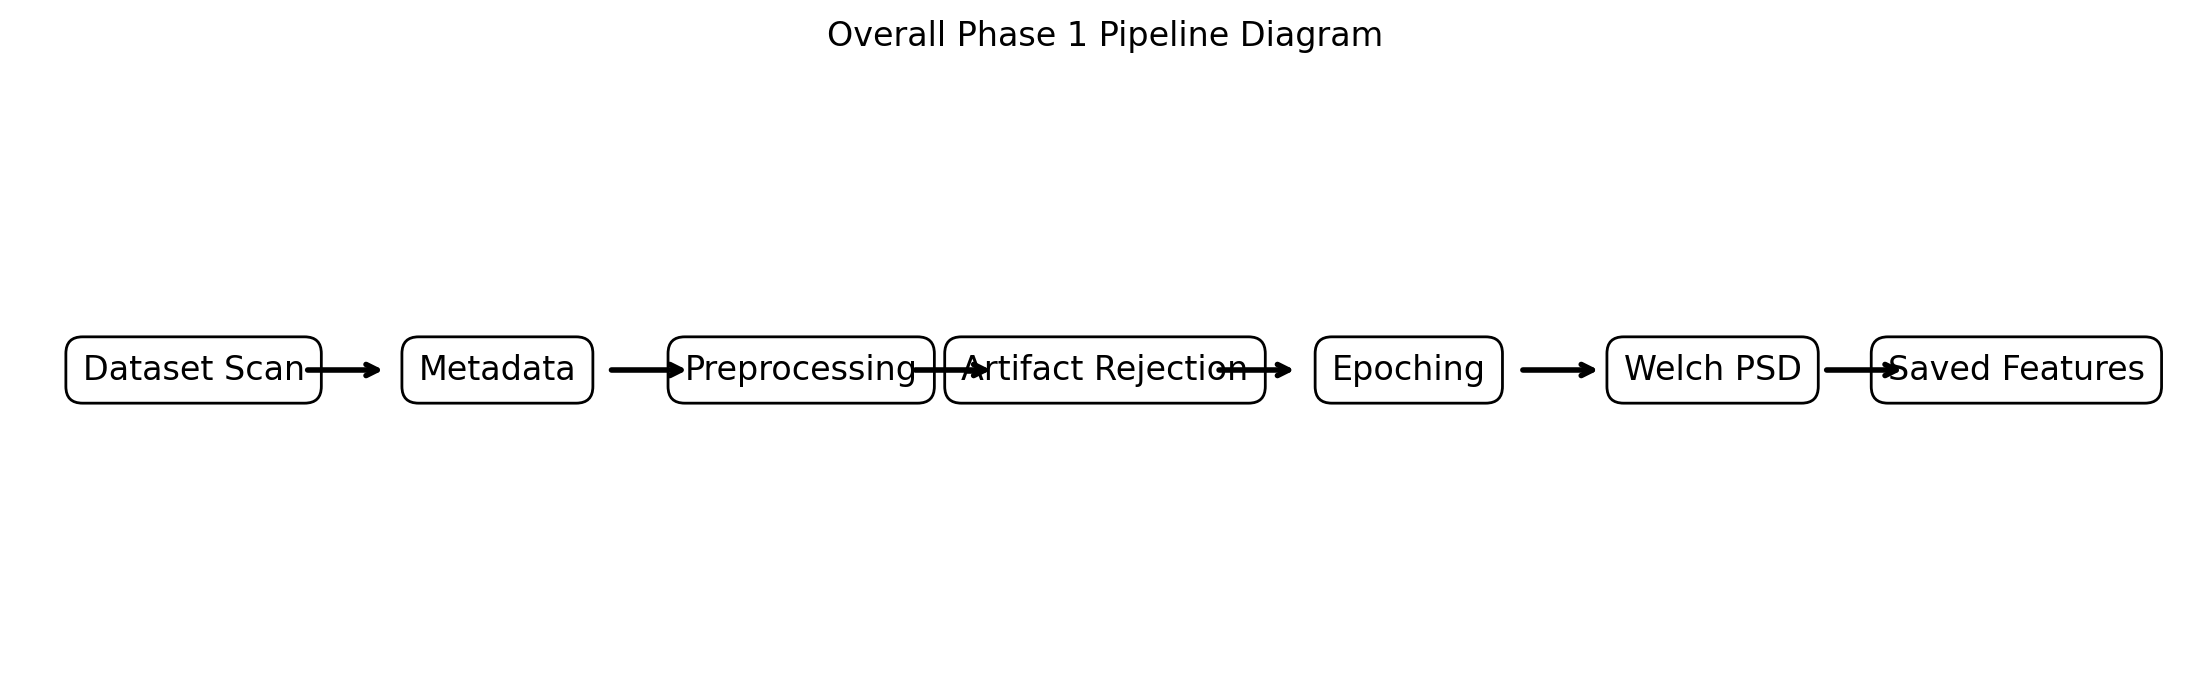
\includegraphics[width=0.9\textwidth]{results/figures/01_pipeline_diagram.png}
\caption{Phase 1 workflow implemented in the current progress stage}
\end{figure}

\subsection{Dataset Acquisition and Inspection}
\textbf{Status: \textcolor{green}{Completed}}

The dataset used in this work is OpenNeuro \texttt{ds004504} \cite{openneuro_ds004504}. EEG files were scanned recursively from the raw data directory and matched with participant information obtained from \texttt{participants.tsv}.

\subsubsection{Dataset Composition}
\begin{itemize}
    \item Total EEG files detected recursively: 176
    \item Total matched subjects: 88
    \item Alzheimer’s Disease (AD): 36 subjects
    \item Cognitively Normal (CN): 29 subjects
    \item Frontotemporal Dementia (FTD): 23 subjects
\end{itemize}

\subsubsection{Recording Specifications}
\begin{itemize}
    \item Recording type: Resting-state eyes-closed EEG
    \item Number of EEG channels: 19
    \item Sampling frequency: approximately 500 Hz
    \item Label mapping used: AD = 0, CN = 1, FTD = 2
\end{itemize}

\begin{figure}[H]
\centering
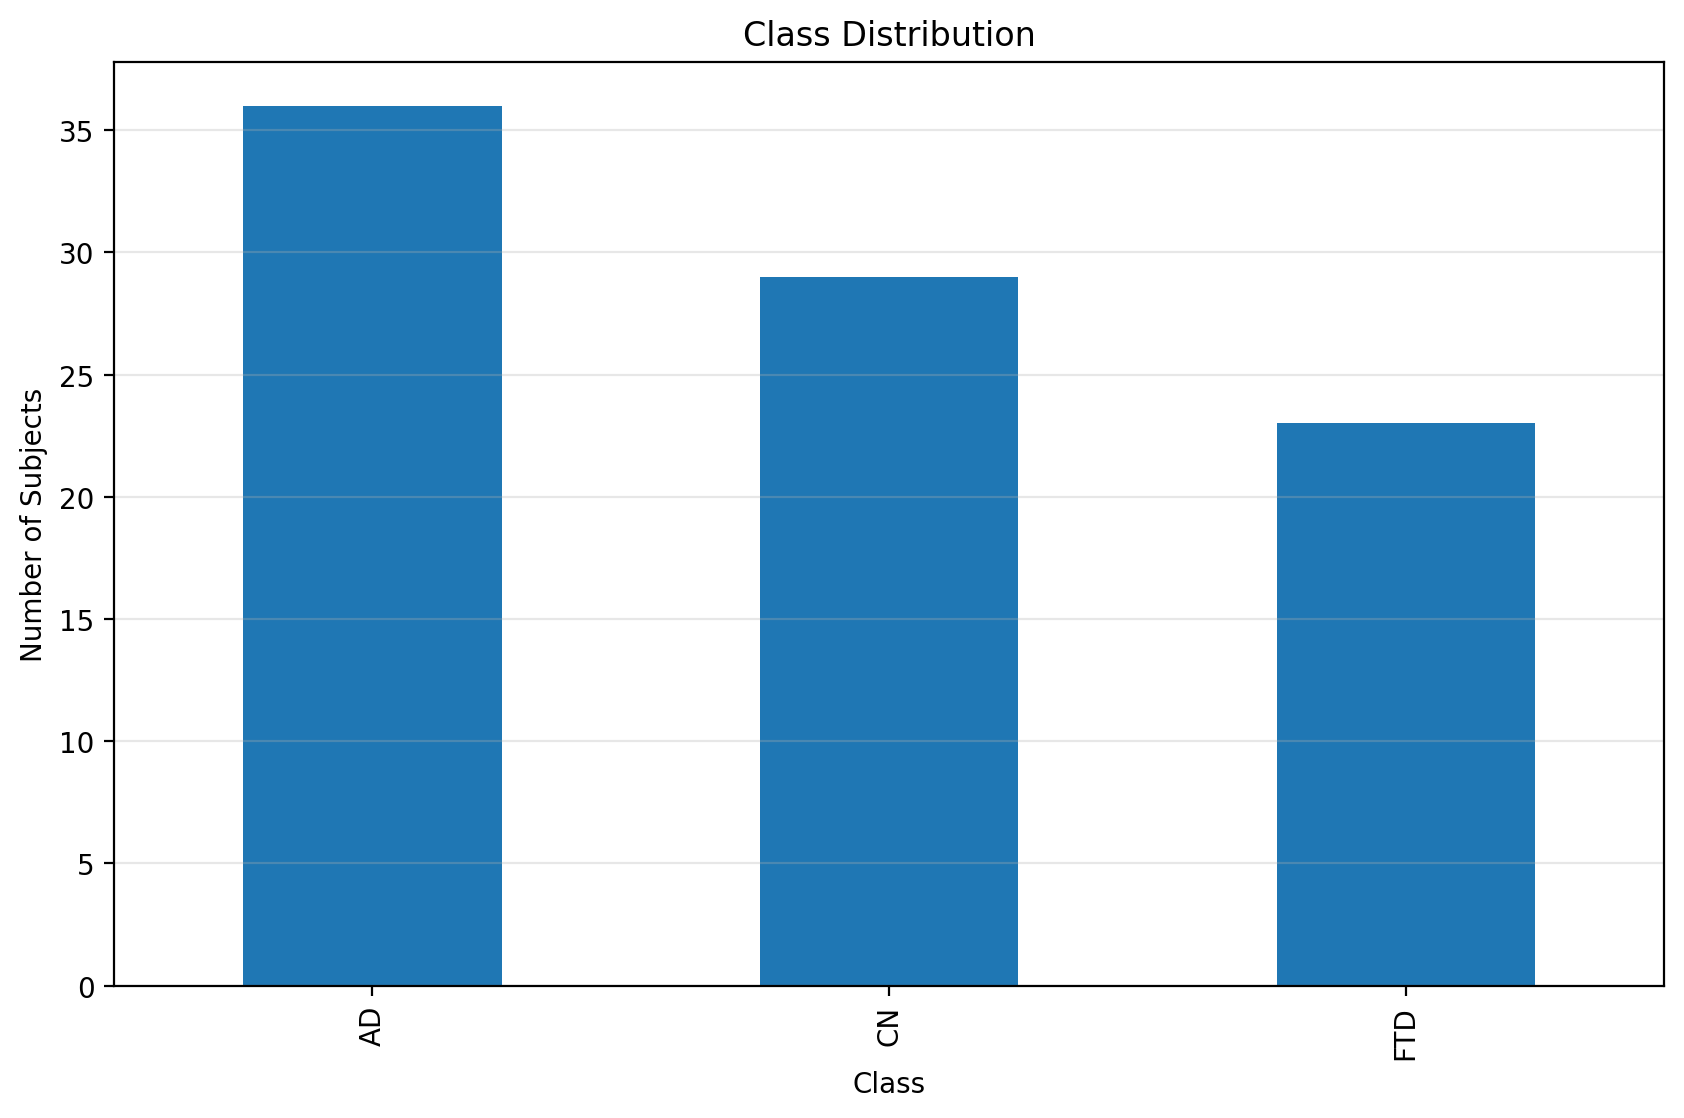
\includegraphics[width=0.7\textwidth]{results/figures/02_class_distribution.png}
\caption{Class distribution of matched subjects in the dataset}
\end{figure}

\subsection{Metadata Creation}
\textbf{Status: \textcolor{green}{Completed}}

After identifying EEG recordings, a structured metadata table was created for all valid subjects. The metadata file contains the following fields:
\begin{itemize}
    \item \texttt{subject\_id}
    \item \texttt{label}
    \item \texttt{class\_name}
    \item \texttt{eeg\_file}
\end{itemize}

This metadata was saved as:
\begin{center}
\texttt{data/metadata/subject\_metadata.csv}
\end{center}

This file acts as the central mapping table for all subsequent preprocessing and feature extraction steps.

\subsection{EEG Preprocessing Pipeline}
\textbf{Status: \textcolor{green}{Completed}}

The preprocessing stage was implemented using the MNE library \cite{gramfort2013}. The goal was to create a fixed and reproducible pipeline that prepares the raw EEG for PSD extraction.

\subsubsection{Step 1: EEG Loading}
EEG recordings were loaded using MNE with support for common EEG formats such as \texttt{.set}, \texttt{.edf}, \texttt{.vhdr}, and \texttt{.fif}. For the current dataset, the valid recordings were loaded from the detected EEG files associated with each subject.

\subsubsection{Step 2: Band-pass Filtering}
A band-pass filter from 0.5 Hz to 45 Hz was applied to each EEG recording. This filtering step was used to:
\begin{itemize}
    \item reduce low-frequency baseline drift and slow fluctuations;
    \item suppress higher-frequency noise outside the target EEG analysis range;
    \item preserve the main EEG spectral content relevant to the present study.
\end{itemize}

\begin{figure}[H]
\centering
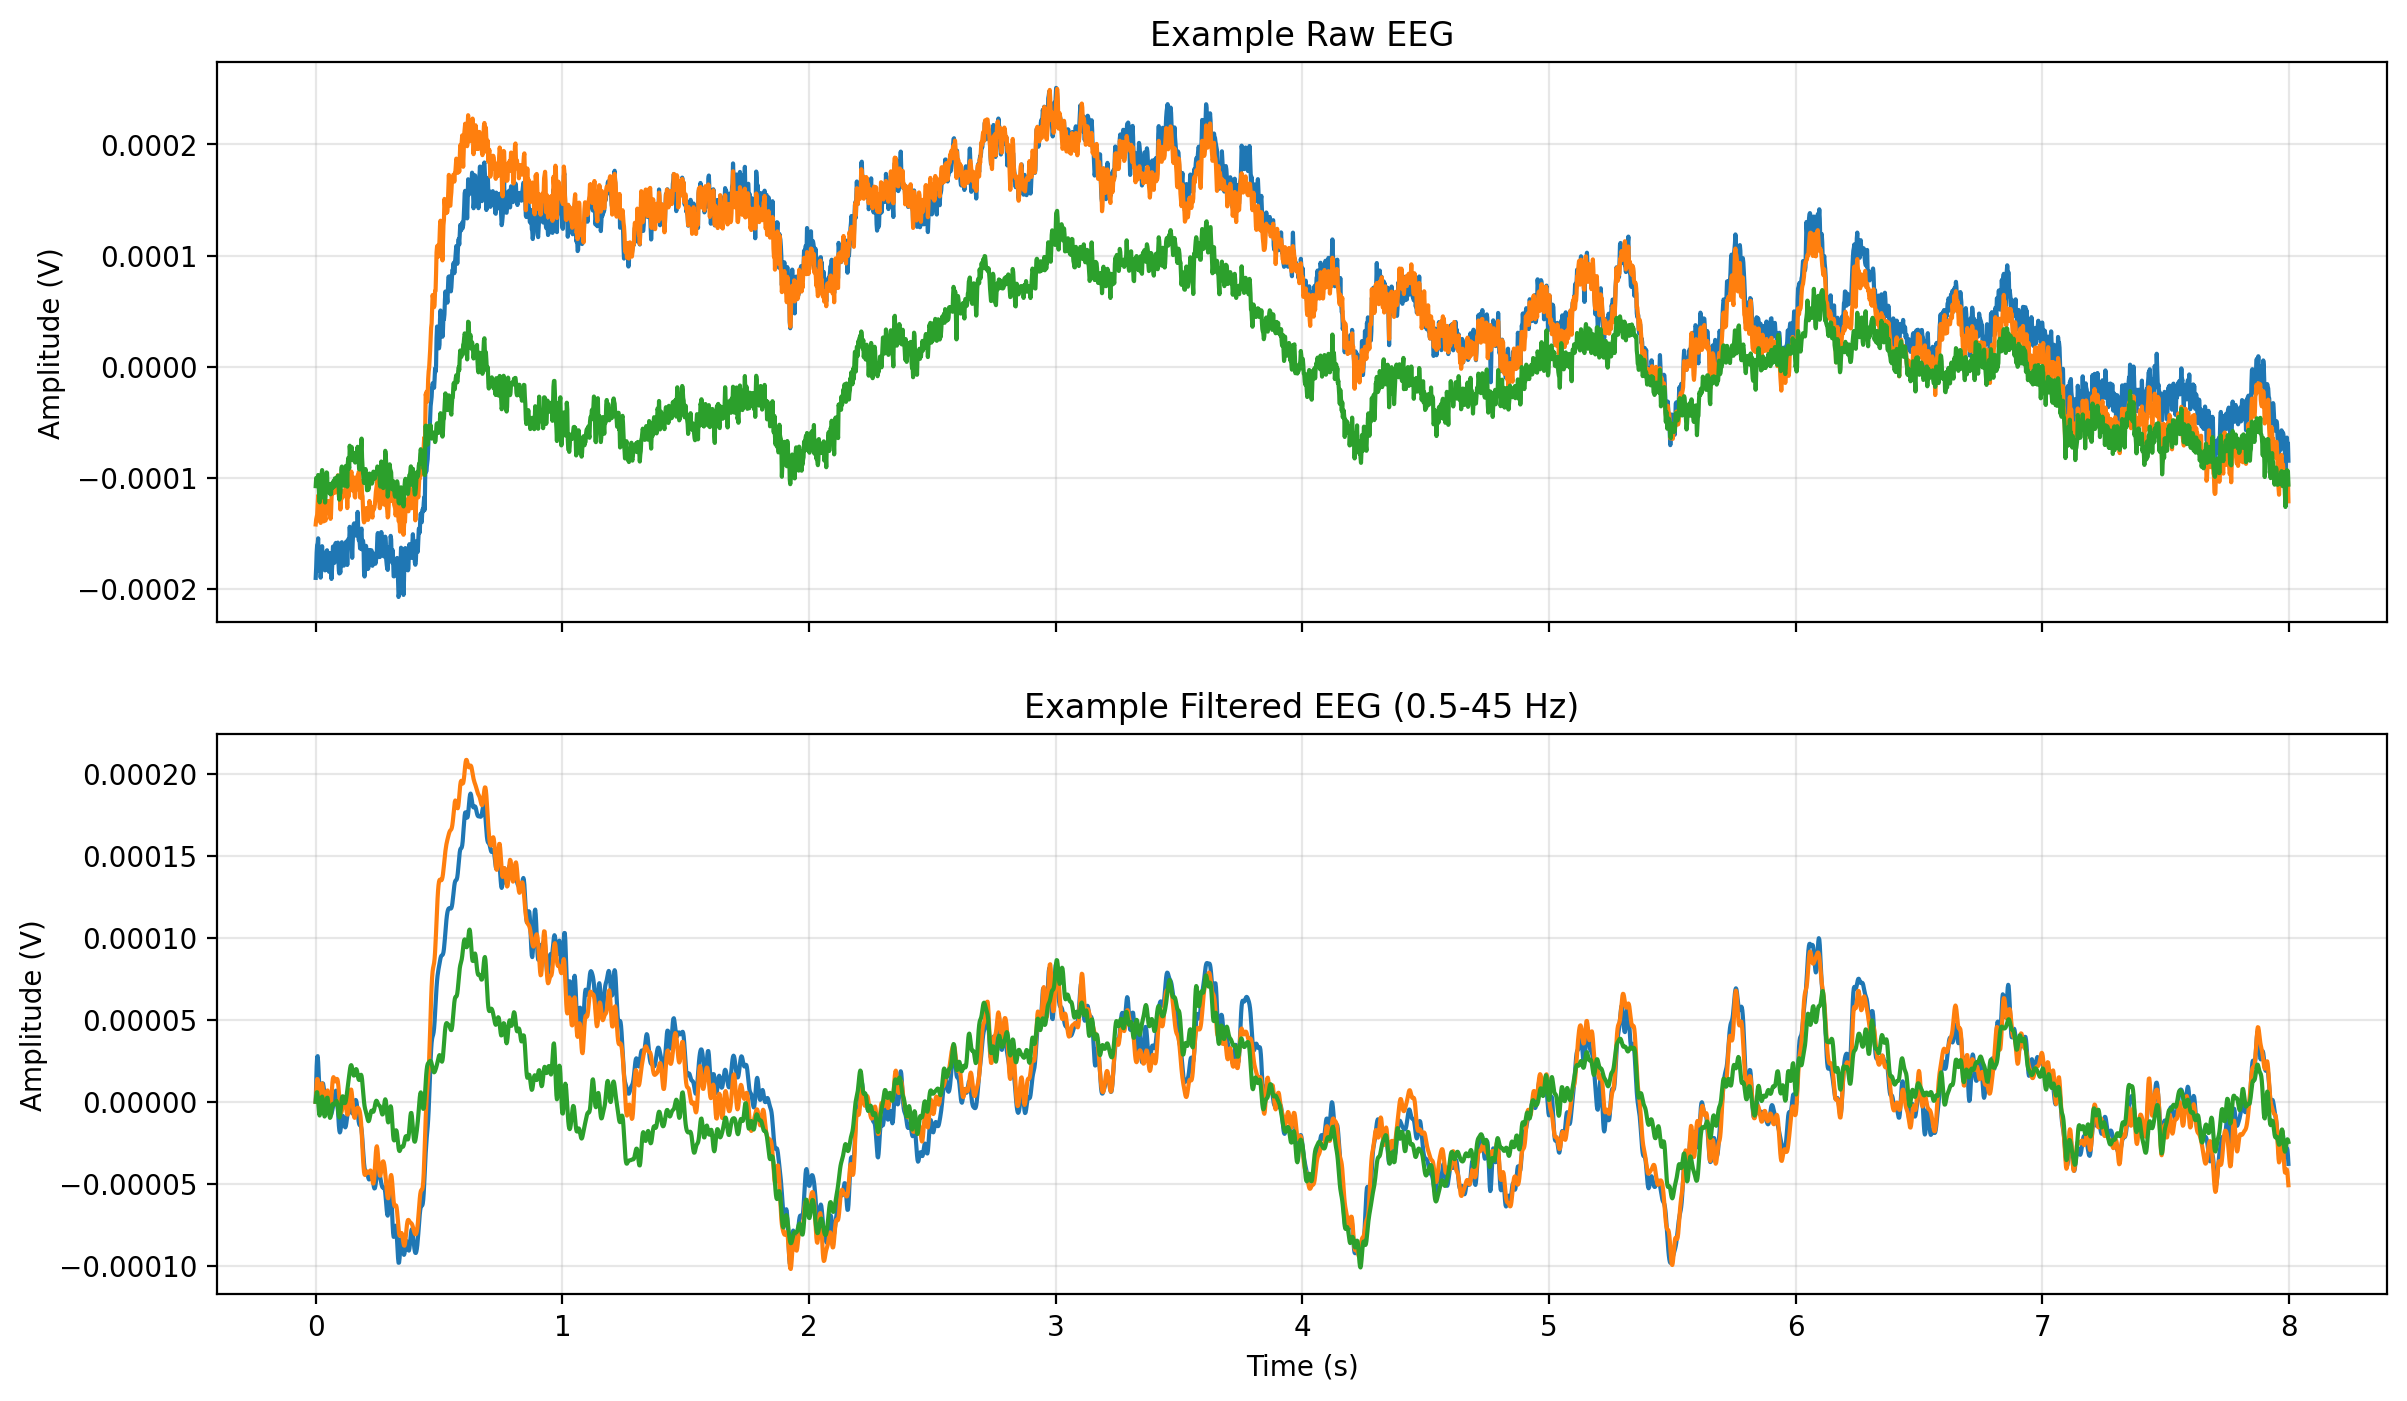
\includegraphics[width=0.95\textwidth]{results/figures/03_raw_vs_filtered_eeg.png}
\caption{Example raw versus filtered EEG signal from the implemented preprocessing pipeline}
\end{figure}

\subsubsection{Step 3: Epoch Segmentation}
After filtering, the continuous EEG signal was segmented into fixed 4-second epochs using two configurations:

\begin{itemize}
    \item Epoch duration: 4 seconds
    \item Non-overlap setting: 0\% overlap (baseline)
    \item Overlap setting: 50\% overlap (2-second shift between consecutive epochs)
    \item Samples per epoch: 2000 at 500 Hz
\end{itemize}

This dual setting was included to evaluate whether overlap increases usable training samples while keeping preprocessing rules fixed and reproducible.

\begin{figure}[H]
\centering
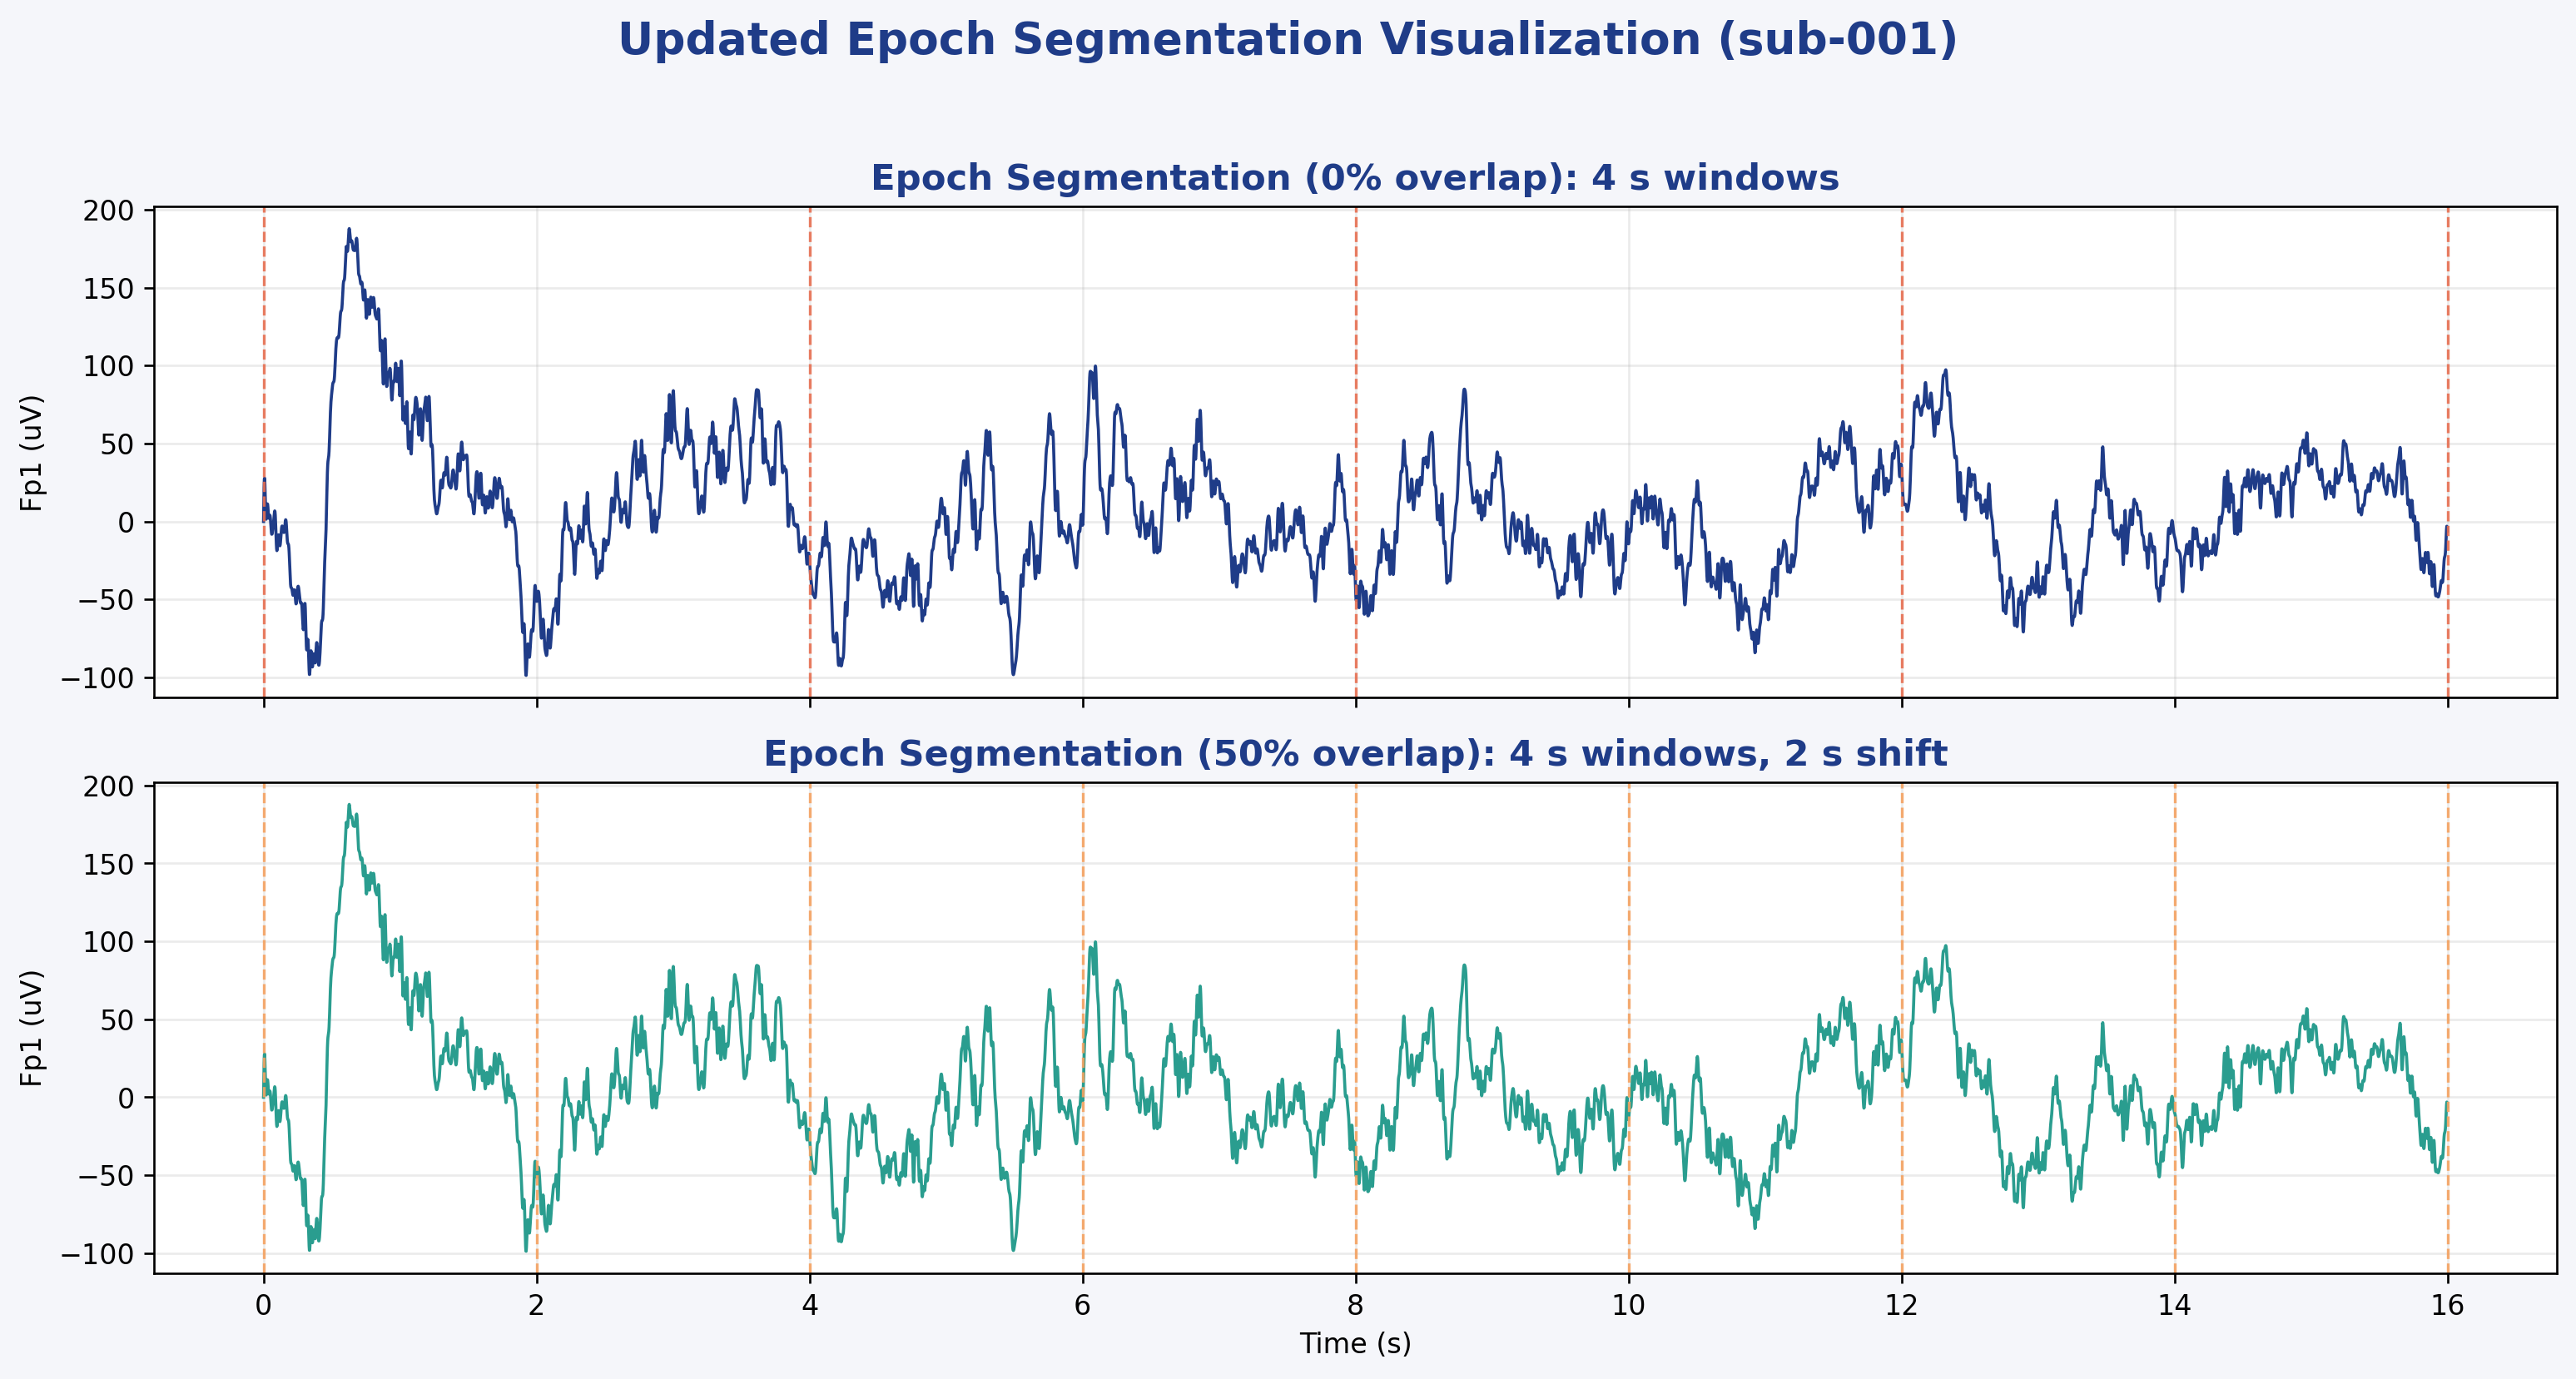
\includegraphics[width=0.95\textwidth]{results/figures/epoch_segmentation_sample.png}
\caption{Example of segmentation into fixed 4-second EEG epochs}
\end{figure}

\subsubsection{Step 4: Artifact Rejection}
Artifact rejection was applied after epoch segmentation. Each epoch was checked using two fixed criteria:
\begin{itemize}
    \item amplitude threshold: $\pm 150\ \mu V$
    \item high-frequency artifact check in the 20--45 Hz band
\end{itemize}

These thresholds were kept fixed and non-tuned in order to maintain a stable baseline preprocessing pipeline for the progress phase.

\begin{figure}[H]
\centering
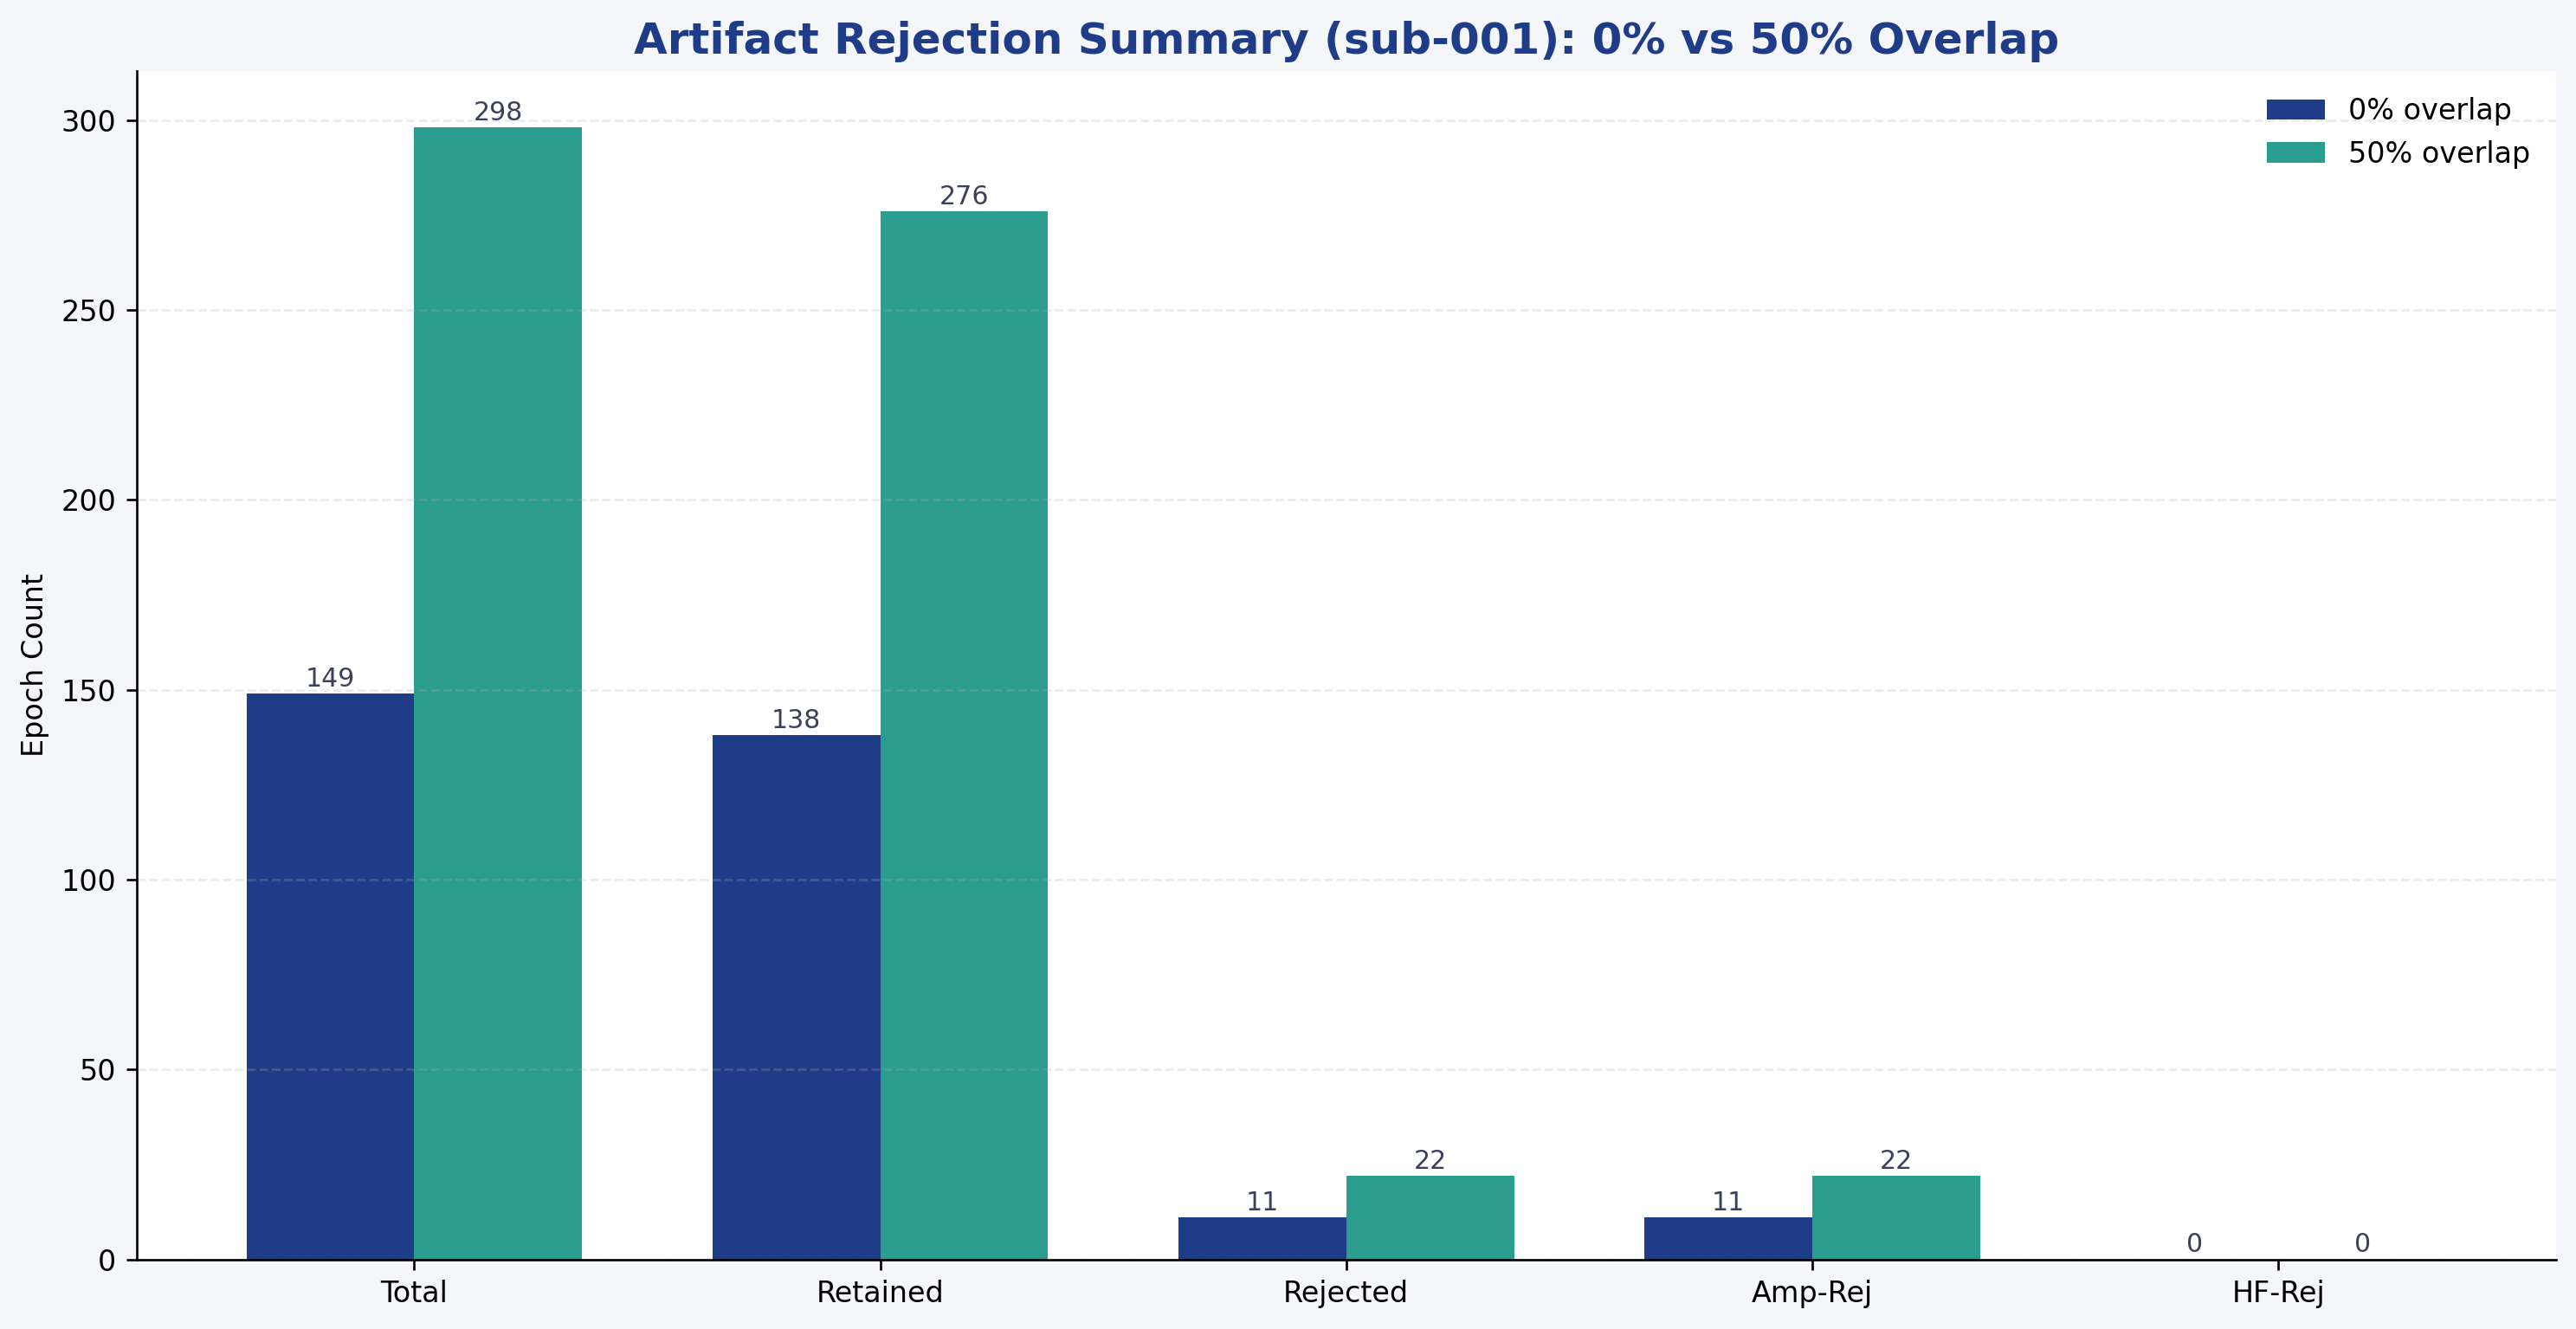
\includegraphics[width=0.8\textwidth]{results/figures/artifact_rejection_sample.png}
\caption{Artifact rejection summary for a sample subject}
\end{figure}

\subsubsection{Example Preprocessing Output}
For the demonstration subject \texttt{sub-001}, the preprocessing stage produced the following verified output:
\begin{itemize}
    \item Sampling frequency: 500 Hz
    \item Number of channels: 19
    \item Retained epochs: 138
    \item Example epoch array shape: \texttt{(138, 19, 2000)}
\end{itemize}

\begin{figure}[H]
\centering
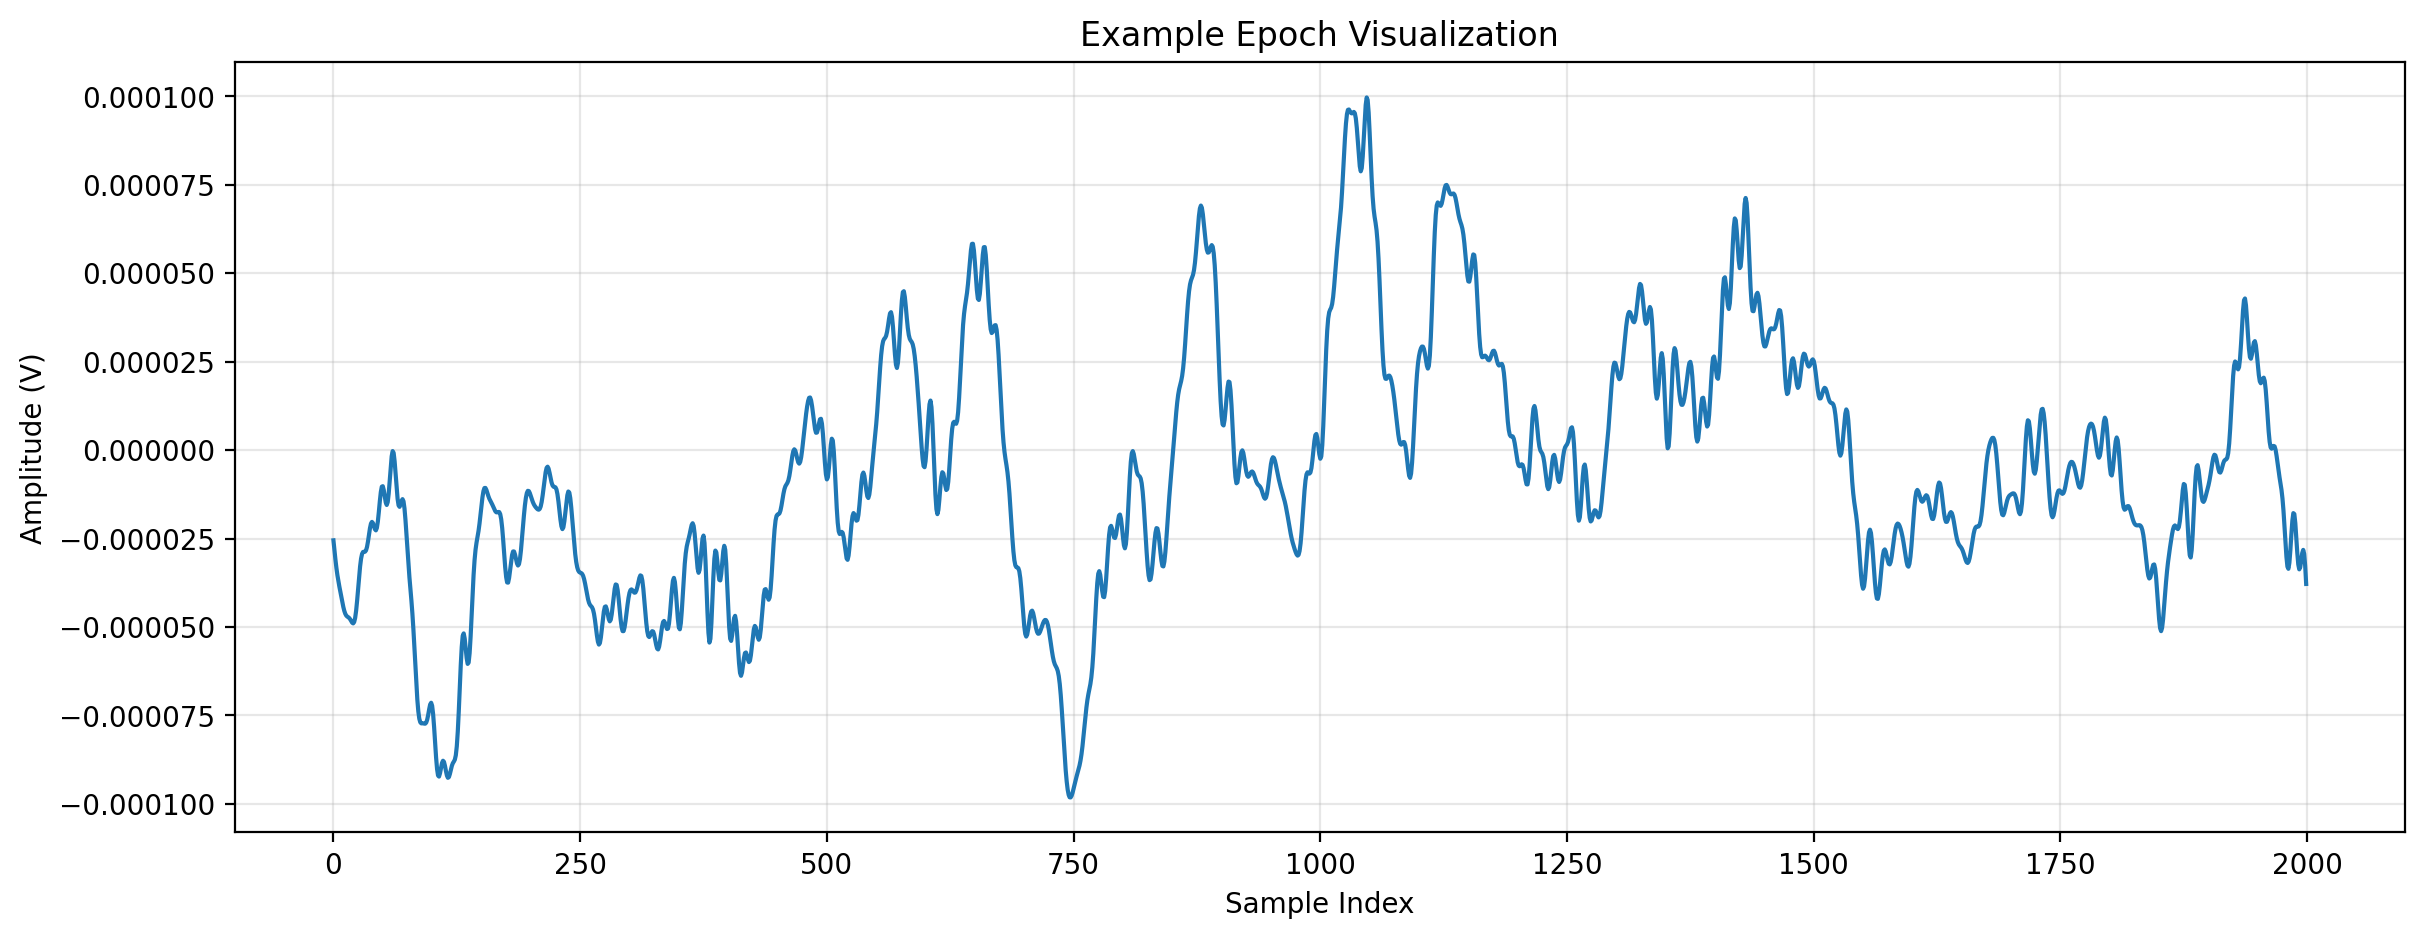
\includegraphics[width=0.85\textwidth]{results/figures/04_example_epoch.png}
\caption{Example retained EEG epoch after preprocessing}
\end{figure}

\subsection{Welch PSD Feature Extraction}
\textbf{Status: \textcolor{green}{Completed}}

The core feature extraction stage in the current project uses Welch Power Spectral Density (PSD) \cite{welch1967}. Welch PSD converts EEG signals into a frequency-domain representation by estimating how signal power is distributed across frequencies.

\subsubsection{Welch PSD Parameters}
The following parameters were used throughout the pipeline:
\begin{itemize}
    \item \texttt{fmin = 1}
    \item \texttt{fmax = 45}
    \item \texttt{n\_fft = 1000}
    \item \texttt{n\_per\_seg = 1000}
    \item \texttt{n\_overlap = 500}
    \item Window: Hamming
\end{itemize}

These settings were chosen to cover the main EEG frequency range, provide 0.5 Hz spectral resolution, and maintain stable PSD estimation across all subjects \cite{welch1967,cassani2018}.

\subsubsection{Mathematical Formulation Used}
The key equations used in preprocessing and feature extraction are:

\textbf{1) Number of epochs from a recording}
\[
N_{\text{epochs}}=\left\lfloor\frac{T-L}{L-O}\right\rfloor+1
\]
where \(T\) is recording length (seconds), \(L\) is epoch length, and \(O\) is overlap.

\textbf{2) Welch PSD estimate}
\[
\hat{P}_{xx}(f)=\frac{1}{K}\sum_{k=1}^{K}\frac{1}{U}\left|\sum_{n=0}^{N-1}x_k[n]\,w[n]\,e^{-j2\pi fn/F_s}\right|^2
\]
where \(K\) is number of segments, \(w[n]\) is the Hamming window, \(F_s\) is sampling frequency, and
\[
U=\frac{1}{N}\sum_{n=0}^{N-1}w^2[n].
\]

\textbf{3) Frequency resolution}
\[
\Delta f=\frac{F_s}{n_{\text{fft}}}.
\]
For this project, \(F_s=500\) Hz and \(n_{\text{fft}}=1000\), so \(\Delta f=0.5\) Hz.

\textbf{4) Relative PSD normalization}
\[
P_{\text{rel}}(f)=\frac{P(f)}{\sum\limits_{f'=f_{\min}}^{f_{\max}}P(f')}.
\]
This normalization removes overall amplitude scale effects and preserves the power distribution across frequencies.

\subsubsection{Normalization}
Relative normalization was applied to the PSD features. This means each PSD estimate was normalized by total power so that the resulting values represent relative power distribution rather than absolute scale.

\subsubsection{Feature Output Shape}
The PSD features were computed in the following shape format:
\begin{center}
\texttt{(n\_epochs, n\_channels, n\_freq\_bins)}
\end{center}

For the demonstration subject \texttt{sub-001}, the verified PSD output shape was:
\begin{center}
\texttt{(138, 19, 89)}
\end{center}

\begin{figure}[H]
\centering
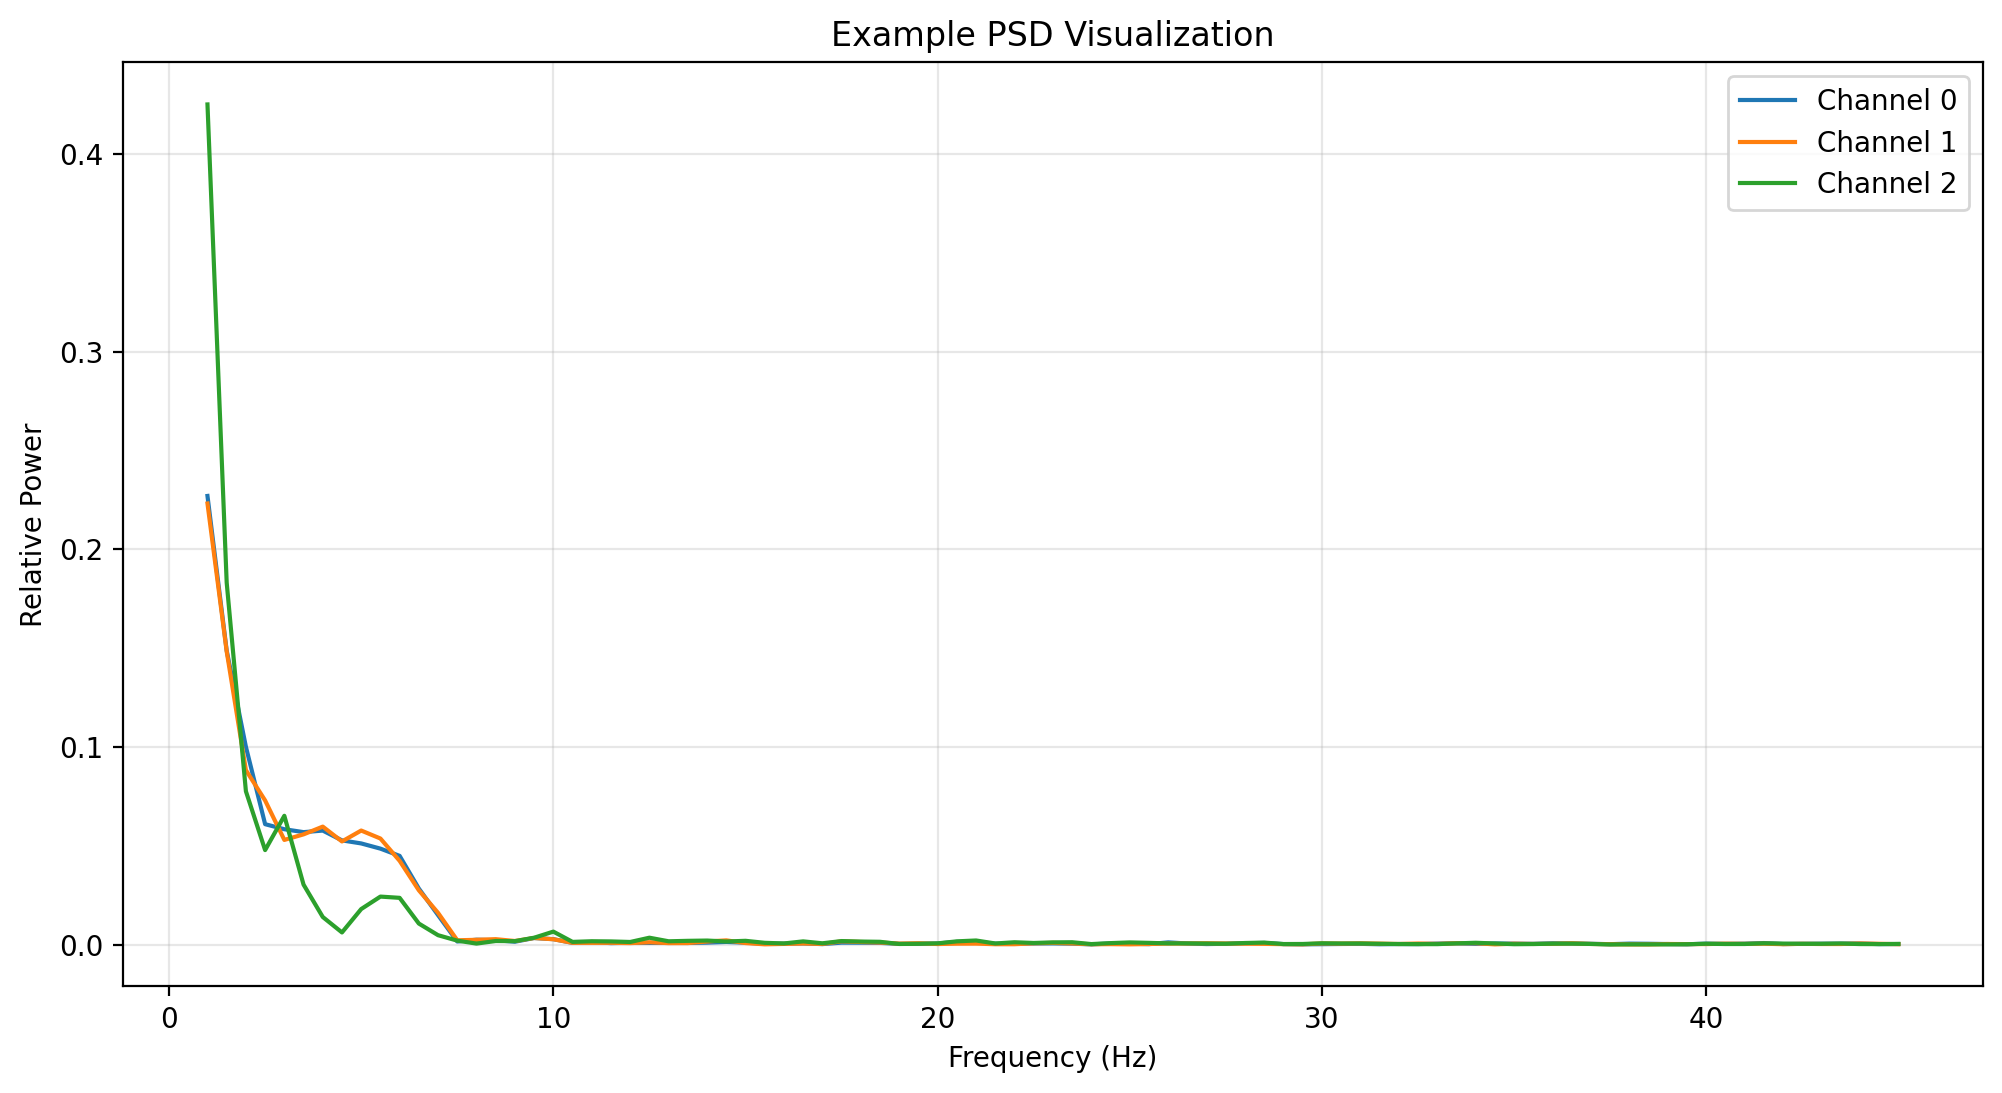
\includegraphics[width=0.85\textwidth]{results/figures/05_example_psd.png}
\caption{Example Welch PSD output from the extracted EEG features}
\end{figure}

\begin{figure}[H]
\centering
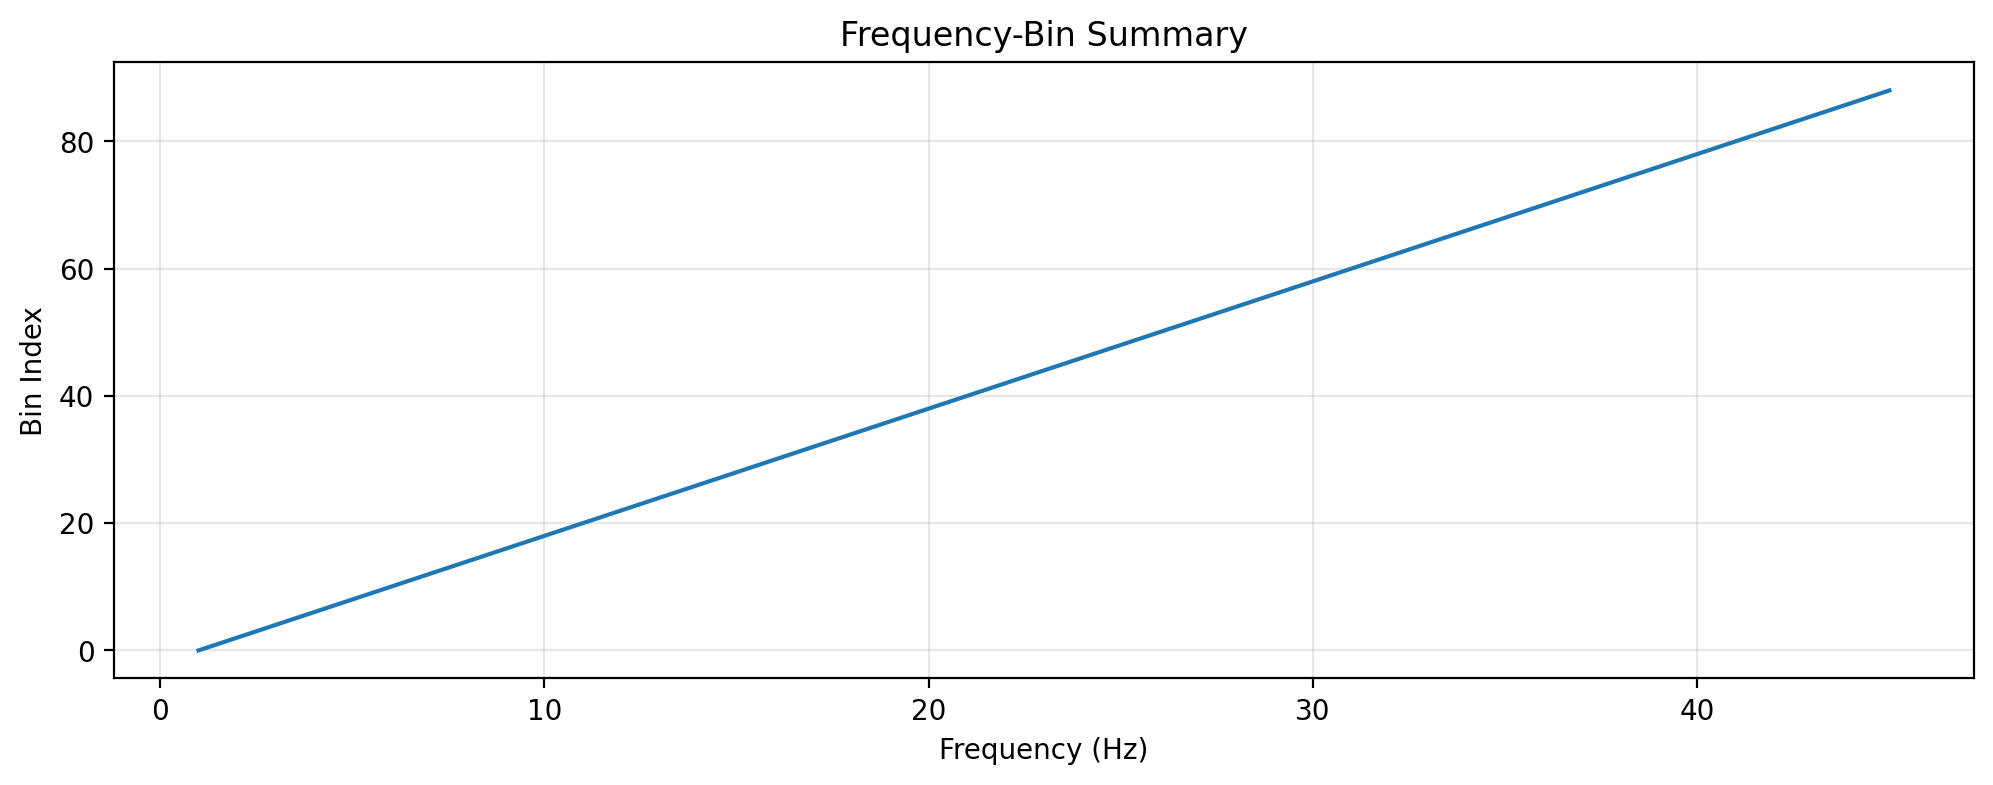
\includegraphics[width=0.85\textwidth]{results/figures/06_frequency_bin_summary.png}
\caption{Frequency analysis range and EEG band interpretation used in Welch PSD}
\end{figure}

\subsubsection{Saved Outputs}
For each valid subject, one PSD feature file was saved in compressed \texttt{.npz} format. Each file contains:
\begin{itemize}
    \item subject ID
    \item class name
    \item numeric label
    \item PSD feature array
    \item frequency vector
\end{itemize}

The subject-wise files were saved under:
\begin{center}
\texttt{data/processed/psd\_features/}
\end{center}

For 50\% overlap, subject-wise files were also saved under:
\begin{center}
\texttt{data/processed/psd\_features\_overlap50/}
\end{center}

In addition, summary files were created:
\begin{center}
\texttt{data/metadata/psd\_feature\_summary.csv} (non-overlap)\\
\texttt{data/metadata/psd\_feature\_summary\_overlap50.csv} (50\% overlap)
\end{center}
These files store the number of retained epochs, number of channels, number of frequency bins, and output file path for each processed subject.

\newpage

% ==================== RESULTS SO FAR ====================
\section{Results Obtained So Far}

\subsection{Dataset and Processing Summary}
The implemented Phase 1 pipeline was executed on the detected valid subjects from the dataset. The verified results obtained so far are:

\begin{table}[H]
\centering
\caption{Phase 1 Processing Summary}
\begin{tabular}{lc}
\toprule
\textbf{Metric} & \textbf{Value} \\
\midrule
Total EEG files detected & 176 \\
Total matched subjects & 88 \\
Successfully processed subjects (both settings) & 88 \\
Failed subjects & 0 \\
Retained epochs per subject (non-overlap) & 163.18 (avg), min 1, max 315 \\
Retained epochs per subject (50\% overlap) & 325.86 (avg), min 5, max 630 \\
Example epoch shape (non-overlap) & \texttt{(138, 19, 2000)} \\
Example PSD shape (non-overlap) & \texttt{(138, 19, 89)} \\
\bottomrule
\end{tabular}
\end{table}

\subsection{Overlap versus Non-overlap Observation}
After implementing both segmentation settings, the 50\% overlap pipeline produced approximately double the average retained epochs per subject (325.86) compared with the non-overlap baseline (163.18), while processing the same 88 subjects successfully. This confirms that overlap can substantially increase sample availability for downstream CNN training.

\subsection{Single-CNN Baseline Preparation}
A pilot EEGNet baseline workflow was added in \texttt{notebooks/06\_single\_cnn\_eegnet\_baseline.ipynb}, with supporting code in \texttt{src/eegnet\_baseline.py}. The notebook prepares subject-level PSD inputs and provides baseline comparison plots for overlap settings:
\begin{itemize}
    \item \texttt{results/figures/10\_eegnet\_accuracy\_bar\_comparison.png}
    \item \texttt{results/figures/11\_eegnet\_accuracy\_dumbbell\_comparison.png}
\end{itemize}

\subsection{Class-wise Processing View}
\begin{figure}[H]
\centering
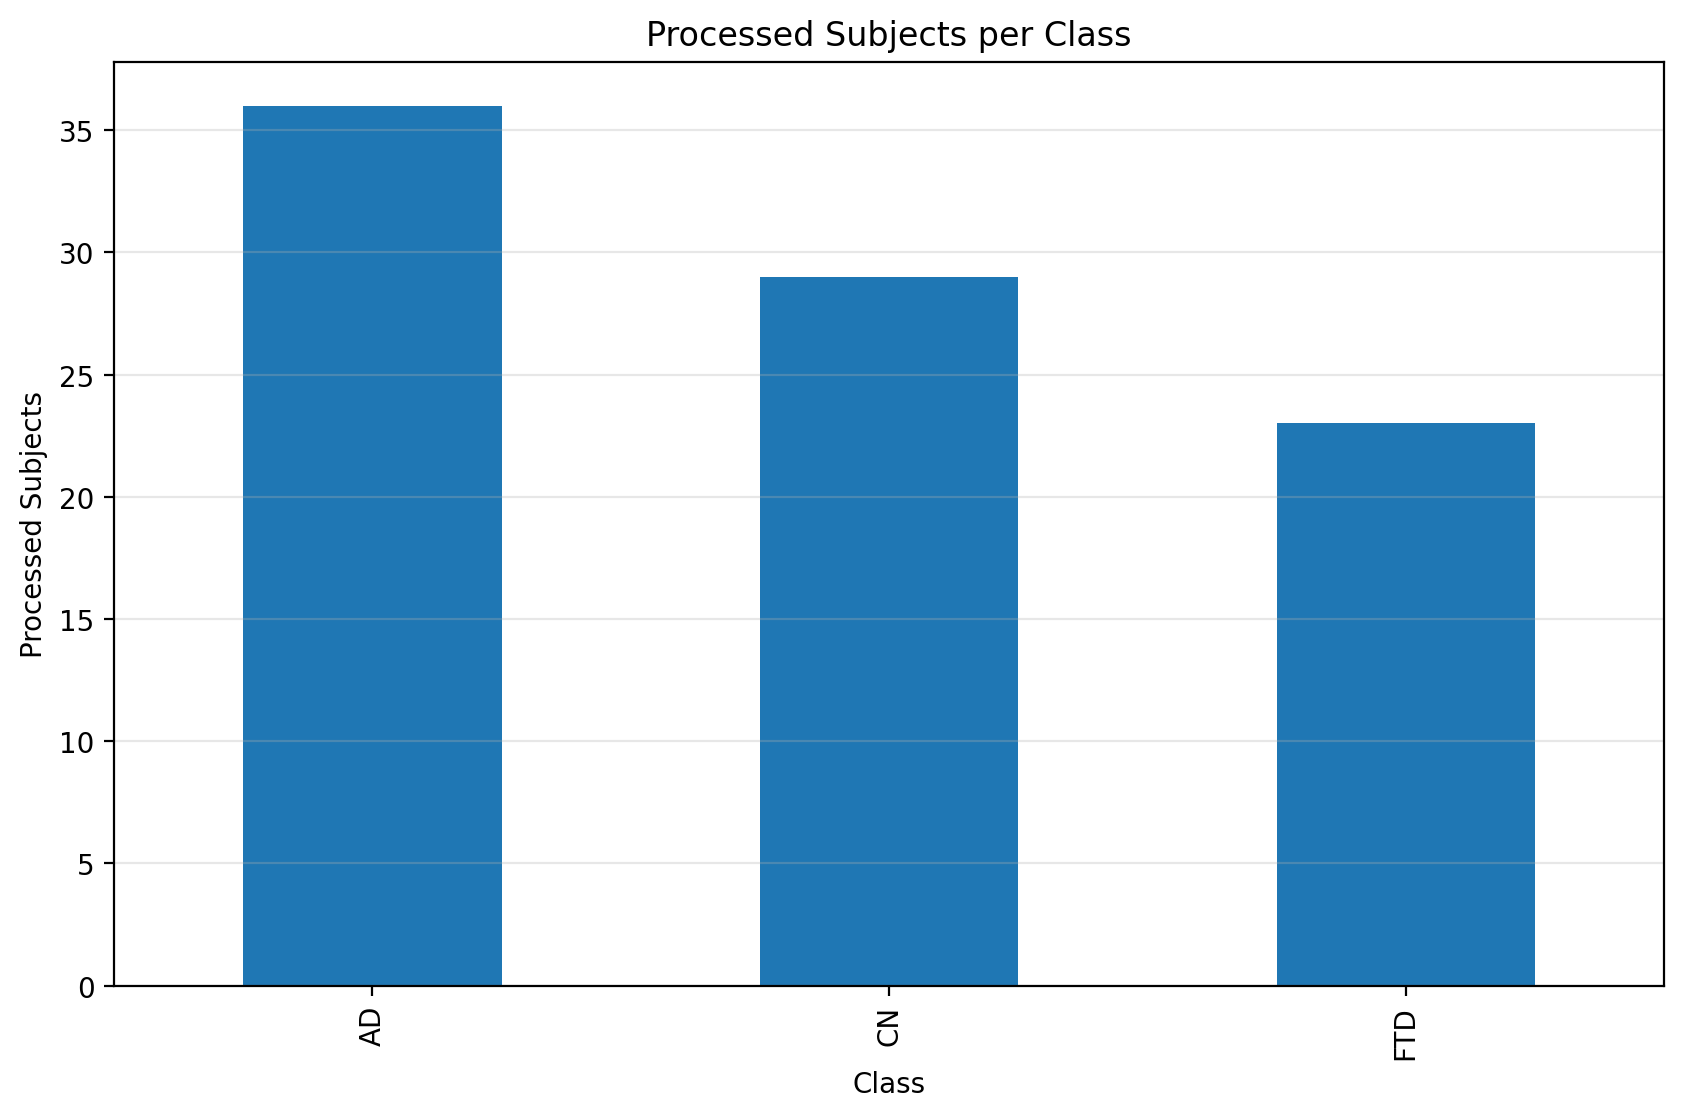
\includegraphics[width=0.75\textwidth]{results/figures/07_processed_subjects_per_class.png}
\caption{Processed subject count by class}
\end{figure}

\subsection{Epoch Count Distribution}
\begin{figure}[H]
\centering
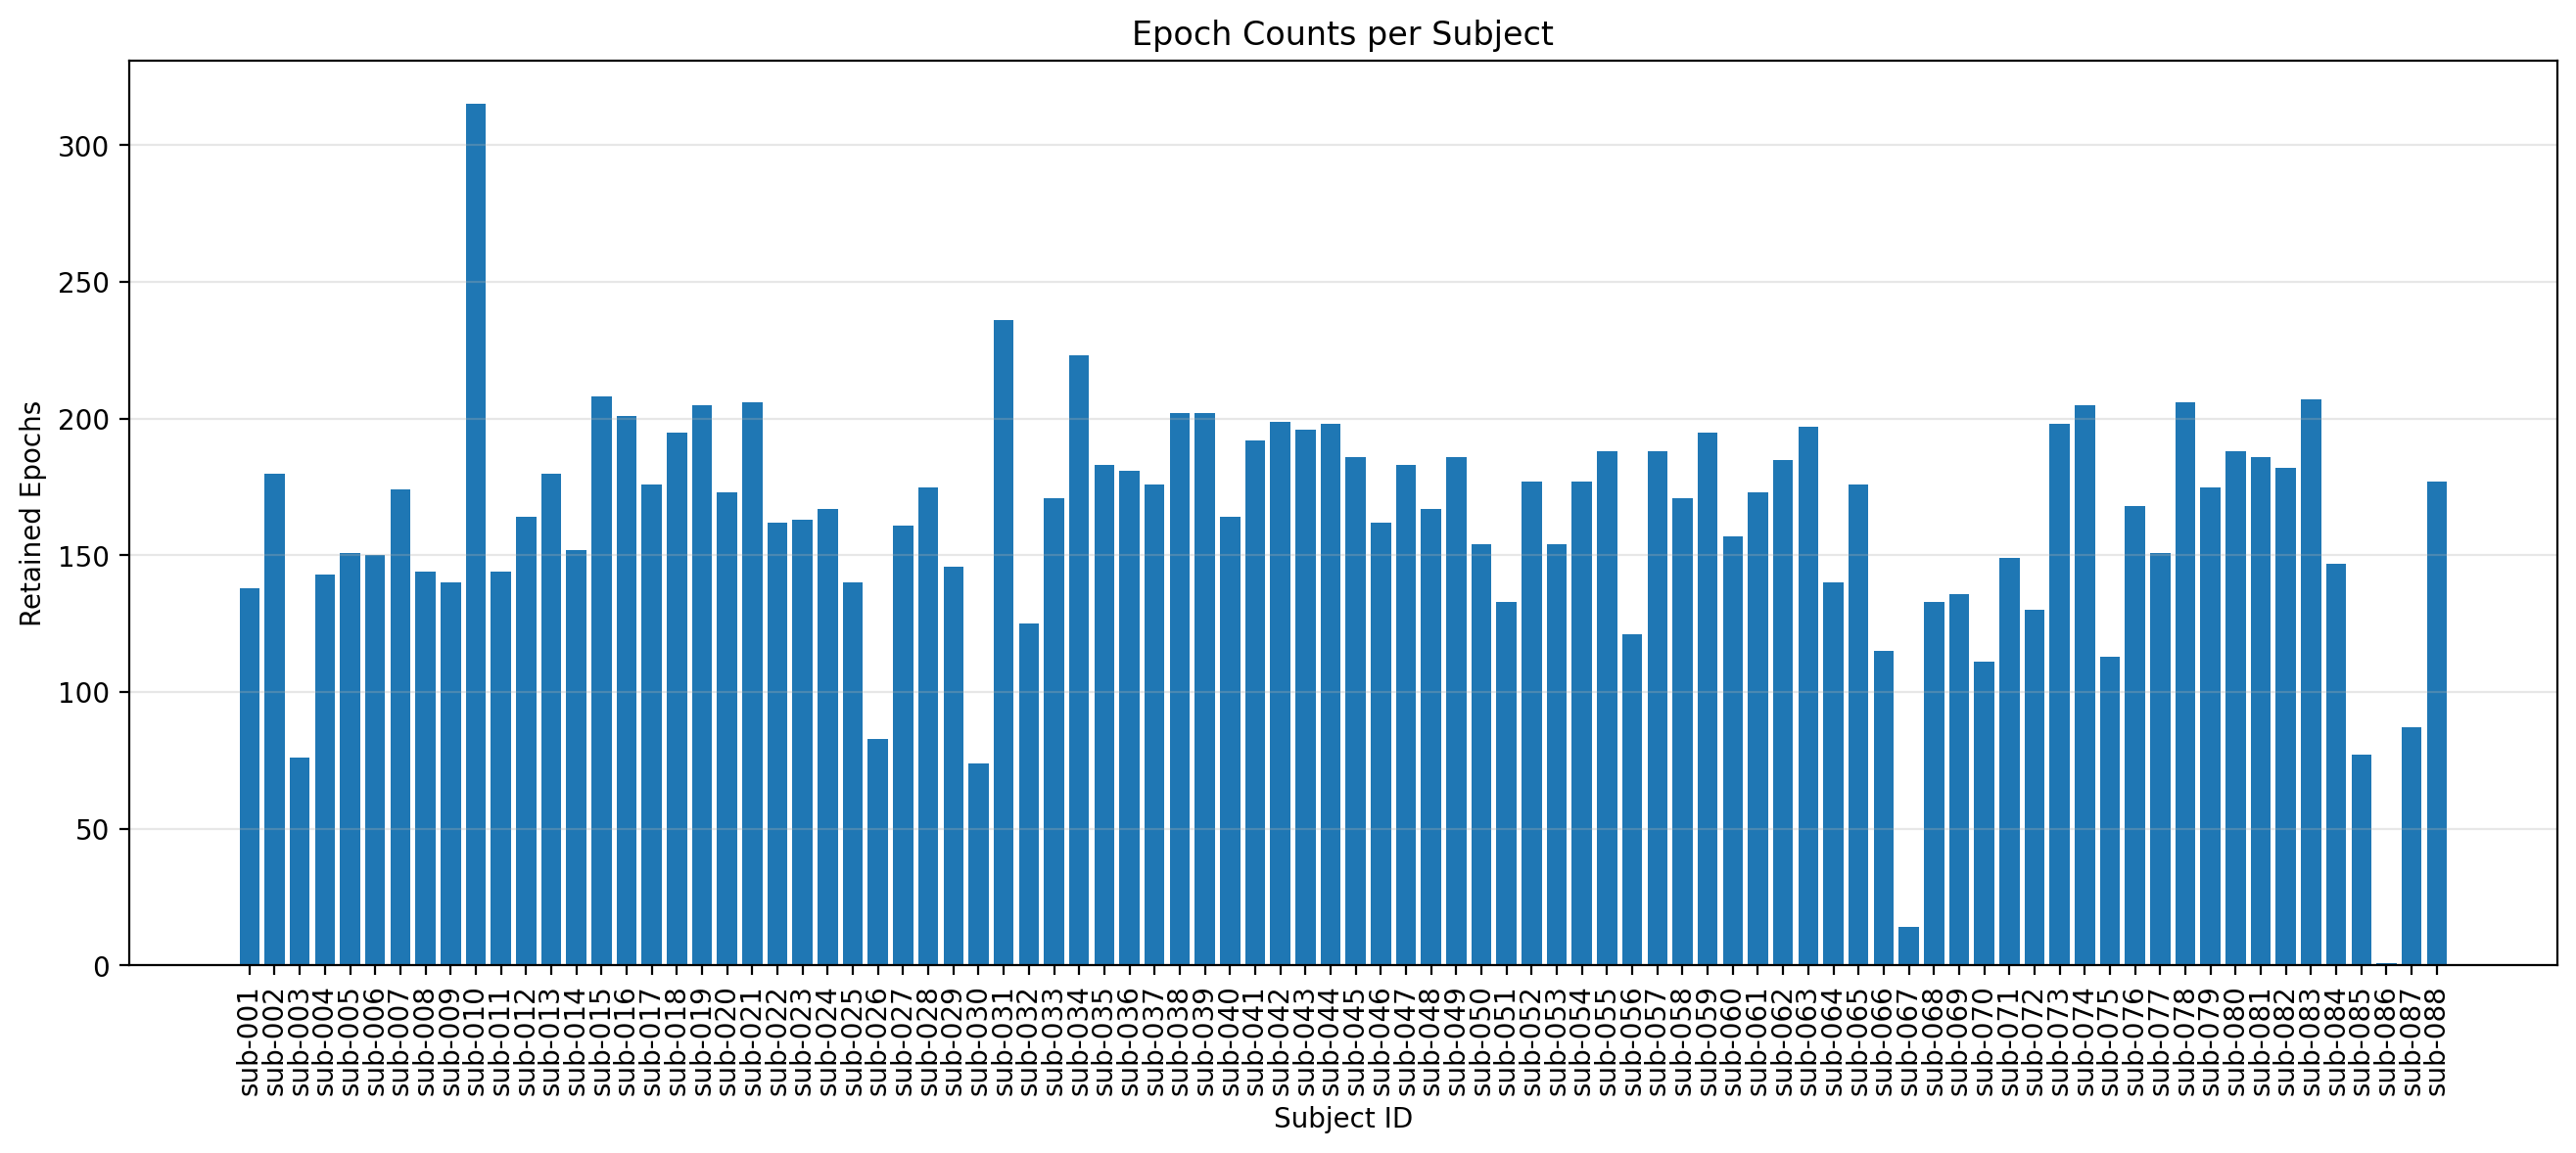
\includegraphics[width=0.95\textwidth]{results/figures/08_epoch_counts_per_subject.png}
\caption{Retained epoch counts across subjects after preprocessing and rejection}
\end{figure}

\subsection{Progress Summary Figure}
\begin{figure}[H]
\centering
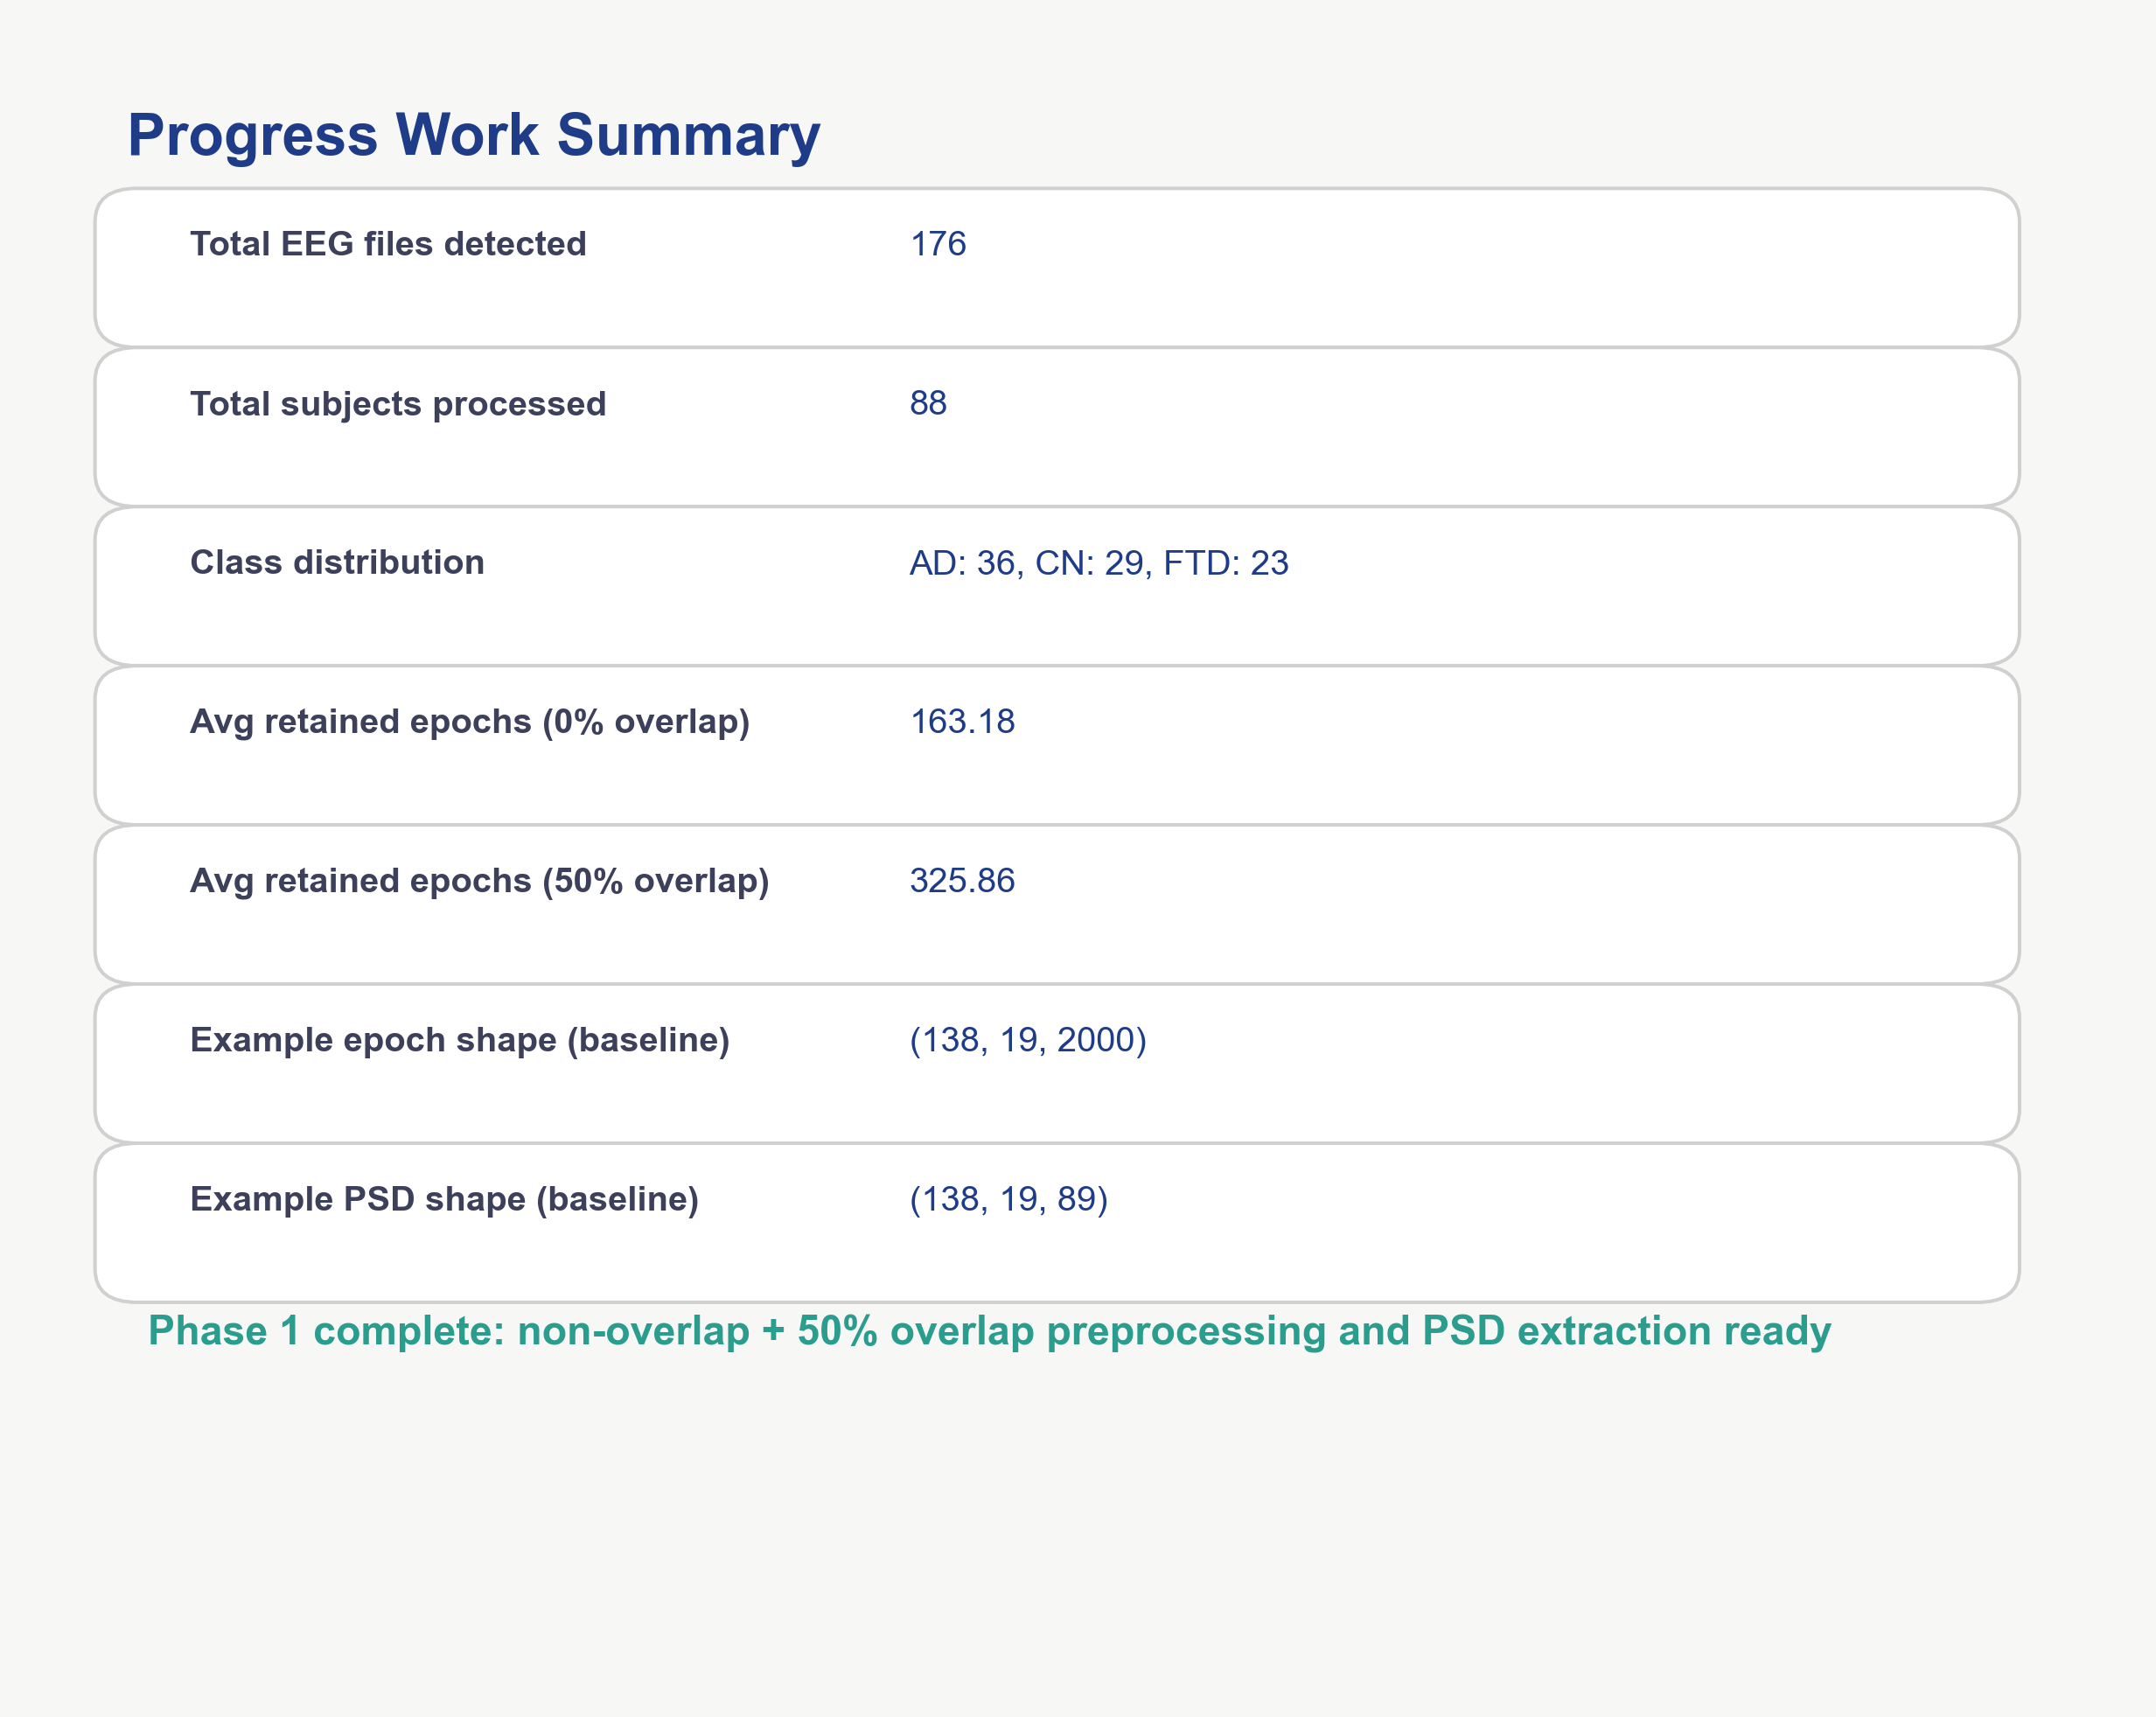
\includegraphics[width=0.85\textwidth]{results/figures/09_progress_work_summary.png}
\caption{Summary of current Phase 1 progress}
\end{figure}

\subsection{Interpretation of Results So Far}
The results show that the implemented Phase 1 pipeline is functioning correctly on the local dataset. The dataset scan detected the expected total of 88 matched subjects, which agrees with the known participant count for this study. All matched subjects were processed successfully without stopping the pipeline.

The retained epoch counts vary across subjects, which is expected due to different artifact levels in real EEG recordings. However, the pipeline still produced valid PSD features for every processed subject. This confirms that the current implementation is stable enough to support the next phase of the thesis, where the extracted features will be used for CNN-based experiments.

\newpage

% ==================== WORK REMAINING ====================
\section{Work Remaining}

\subsection{Phase 2 Tasks}
The following tasks remain for the final phase of the thesis:
\begin{itemize}
    \item prepare subject-wise train, validation, and test splits;
    \item apply stratified or group-aware evaluation design to prevent data leakage;
    \item finalize EEGNet baseline training and evaluation runs;
    \item implement remaining CNN models: ShallowConvNet, DeepConvNet, SCCNet, and FBCNet;
    \item load saved PSD features as inputs for model training;
    \item train all selected models under a common experimental setup;
    \item evaluate model performance using metrics such as accuracy, precision, recall, F1-score, and related measures;
    \item compare model performance and identify the most effective CNN architecture for this task.
\end{itemize}

\subsection{Expected Outcome of Future Phase}
The next phase will transform the extracted PSD features into a reproducible model comparison framework. The final outcome of the thesis will be a comparative evaluation of multiple CNN architectures for Alzheimer’s disease related EEG classification using a shared Welch PSD feature representation.

\newpage

% ==================== CONCLUSION ====================
\section{Conclusion}

This progress report documents the successful completion of the first major phase of the thesis work. The current implementation includes:
\begin{itemize}
    \item dataset inspection and recursive EEG file detection;
    \item metadata creation and subject-label mapping;
    \item EEG loading and filtering using MNE;
    \item fixed-length epoch segmentation with both 0\% overlap and 50\% overlap settings;
    \item artifact rejection using fixed thresholds;
    \item Welch PSD feature extraction;
    \item saving subject-wise features and summary outputs for both segmentation settings;
    \item pilot EEGNet baseline workflow integration for Phase 2 readiness;
    \item generation of progress-ready figures and visual summaries.
\end{itemize}

The most important outcome of this stage is that a clean, modular, and verified EEG feature extraction pipeline is now available for all valid subjects in the dataset under both segmentation settings. Since the current stage processed 88 matched subjects successfully and produced reusable PSD features, with an initial EEGNet baseline workflow prepared, the work is now ready to proceed into full CNN-based comparative modeling.

\newpage

% ==================== REFERENCES ====================
\section{References}

\begin{thebibliography}{99}

\bibitem{lawhern2018}
Lawhern, V. J., Solon, A. J., Waytowich, N. R., Gordon, S. M., Hung, C. P., \& Lance, B. J. (2018). EEGNet: A compact convolutional neural network for EEG-based brain-computer interfaces. \textit{Journal of Neural Engineering}, 15(5), 056013.

\bibitem{schirrmeister2017}
Schirrmeister, R. T., Springenberg, J. T., Fiederer, L. D. J., Glasstetter, M., Eggensperger, K., Tangermann, M., Hutter, F., Burgard, W., \& Ball, T. (2017). Deep learning with convolutional neural networks for EEG decoding and visualization. \textit{Human Brain Mapping}, 38(11), 5391--5420.

\bibitem{hsu2018}
Hsu, Y. H., Chuang, Y. Y., \& Huang, C. Y. (2018). SCCNet: Spatial component-wise convolutional network for motor-imagery EEG classification. In \textit{2018 IEEE International Conference on Systems, Man, and Cybernetics}.

\bibitem{mane2021}
Mane, R., Chew, E., Chua, K., Ang, K. K., Robinson, N., Vinod, A. P., \& Guan, C. (2021). FBCNet: A multi-view convolutional neural network for brain-computer interface. \textit{arXiv preprint arXiv:2104.01233}.

\bibitem{welch1967}
Welch, P. D. (1967). The use of fast Fourier transform for the estimation of power spectra: A method based on time averaging over short, modified periodograms. \textit{IEEE Transactions on Audio and Electroacoustics}, 15(2), 70--73.

\bibitem{miltiadous2023dataset}
Miltiadous, A., Tzimourta, K. D., Afrantou, T., Giannakeas, N., Tzallas, A. T., Tsipouras, M. G., \& Tsalikakis, D. (2023). A dataset of EEG recordings from Alzheimer’s disease, frontotemporal dementia and healthy subjects.

\bibitem{cassani2018}
Cassani, R., Estarellas, M., San-Martín, R., Fraga, F. J., \& Falk, T. H. (2018). Systematic review on resting-state EEG for Alzheimer’s disease diagnosis. \textit{Disease Markers}, 2018, 5174815.

\bibitem{tzimourta2019}
Tzimourta, K. D., Giannakeas, N., Tzallas, A. T., Tsipouras, M. G., \& Astrakas, L. G. (2019). EEG-based detection of Alzheimer’s disease using machine learning techniques.

\bibitem{fraga2013}
Fraga, F. J., Falk, T. H., Kanda, P. A. M., \& Anghinah, R. (2013). Characterizing Alzheimer’s disease severity using resting-awake EEG amplitude modulation analysis.

\bibitem{tzallas2009}
Tzallas, A. T., Tsipouras, M. G., \& Fotiadis, D. I. (2009). Epileptic seizure detection in EEG signals using time-frequency analysis.

\bibitem{roy2019}
Roy, Y., Banville, H., Albuquerque, I., Gramfort, A., Falk, T. H., \& Faubert, J. (2019). Deep learning-based electroencephalography analysis: A systematic review.

\bibitem{craik2019}
Craik, A., He, Y., \& Contreras-Vidal, J. L. (2019). Deep learning for electroencephalogram classification: A review. \textit{Journal of Neural Engineering}, 16(3), 031001.

\bibitem{gramfort2013}
Gramfort, A., Luessi, M., Larson, E., Engemann, D. A., Strohmeier, D., Brodbeck, C., Goj, R., Jas, M., Brooks, T., Parkkonen, L., \& H\"am\"al\"ainen, M. S. (2013). MEG and EEG data analysis with MNE-Python. \textit{Frontiers in Neuroscience}, 7, 267.

\bibitem{delorme2004}
Delorme, A., \& Makeig, S. (2004). EEGLAB: An open source toolbox for analysis of single-trial EEG dynamics including independent component analysis. \textit{Journal of Neuroscience Methods}, 134(1), 9--21.

\bibitem{jeong2004}
Jeong, J. (2004). EEG dynamics in patients with Alzheimer’s disease. \textit{Clinical Neurophysiology}, 115(7), 1490--1505.

\bibitem{dauwels2010}
Dauwels, J., Vialatte, F., \& Cichocki, A. (2010). Diagnosis of Alzheimer’s disease from EEG signals: Where are we standing? \textit{Current Alzheimer Research}, 7(6), 487--505.

\bibitem{openneuro_ds004504}
OpenNeuro Dataset \texttt{ds004504}. EEG recordings from Alzheimer’s disease, frontotemporal dementia, and healthy subjects. Available at: \url{https://openneuro.org}.

\end{thebibliography}

\end{document}
